% SSR 2026 wrapper (Security Standardisation Research, Baltimore, Dec 13--15 2026).
% BEST near-term fit: the venue is literally about how security standards are
% implemented in the wild, and it accepts Regular / SoK / *Vision* papers — a
% Vision paper honestly fits our current preliminary-measurement-plus-agenda state.
% Open in Overleaf with the Springer LNCS template (llncs.cls).
%   Site: https://ssresearch26.umbc.edu/   CFP: https://cfp.sciltp.com/security-standardisation-research-ssr-conference-2026/
% Rules: <=23 pp LNCS incl. references (appendices don't count); double-blind.
% Deadline 2026-09-15 (AoE). CONFIRM.
\documentclass[runningheads]{llncs}
\usepackage{pgfplots}\pgfplotsset{compat=1.18}
\usepackage{booktabs}
\usepackage[hidelinks]{hyperref}

\title{Authorization Contracts in the Wild: Measuring JWT Verification
Configuration at Scale}
\titlerunning{Authorization Contracts in the Wild}

% Double-blind: anonymous for submission. Camera-ready: Archit Sharma, Garima Mann.
\author{Anonymous Submission (double-blind review)}
\institute{}

\begin{document}
\maketitle
% For SSR, consider the "Vision paper" track if the hand-labelled validation is
% not yet complete by the deadline — it is the honest home for forward-looking work.
% Shared body for the Paper A measurement study. Class-agnostic: the per-venue
% main.tex sets \documentclass, title, authors, and \begin{document}, then
% % Shared body for the Paper A measurement study. Class-agnostic: the per-venue
% main.tex sets \documentclass, title, authors, and \begin{document}, then
% % Shared body for the Paper A measurement study. Class-agnostic: the per-venue
% main.tex sets \documentclass, title, authors, and \begin{document}, then
% \input{../common/body}. Every unfinished number is wrapped in \gate{...}.
% Submission vs. working-copy rendering. Default: submission (clean prose). A
% wrapper can predefine \submissionfalse before \input{../common/body} to bring
% back the loud [PENDING]/[NOTE] markers for internal tracking.
\ifdefined\ifsubmission\else\expandafter\newif\csname ifsubmission\endcsname\submissiontrue\fi
% \gate{...}: forward-looking text. Submission -> plain prose; draft -> [PENDING].
% Content is written to read as a finished future-work sentence either way.
\providecommand{\gate}[1]{\ifsubmission #1\else \textbf{[PENDING: #1]}\fi}
% \draftonly{...}: internal note. Submission -> nothing; draft -> [NOTE].
\providecommand{\draftonly}[1]{\ifsubmission\else \textbf{[NOTE: #1]}\fi}
% Let TeX relax line breaking on paragraphs with long unbreakable \texttt{} kind
% names (RequestAuthentication, AuthorizationPolicy) instead of overrunning the
% margin. Class-agnostic; applies under every venue wrapper.
\emergencystretch=3em

\begin{abstract}
Whether a service accepts a bearer token comes down to configuration, not code:
which issuers it trusts, which audiences it binds to, which algorithms it allows,
and which claims it requires. These settings are spread across service meshes,
proxies, and identity providers, they are rarely written down in one place, and a
single change (a rotated key, a widened audience, a dropped claim) silently turns
valid users away or starts admitting tokens that should be refused. We call this
configuration a service's implicit \emph{authorization contract}, and we think it
should be measured directly rather than assumed. We give a method that derives the
contract from deployment configuration and run it over 428 public repositories. In a
first sample of 102 JWT-validating configurations, none pinned a signing algorithm
in configuration (100\%, leaving it to the verifying library's default), 85.3\%
required no claims, and 42.2\% left the token audience unbound, all with Wilson
95\% confidence intervals. Because a measurement is only as good as its extractor,
we validate it two ways and state each method's limits: a kind-aware oracle for
recall (issuers 89.6\%, audiences 99.0\%), and a negative control for precision that
plants values a correct tool must ignore. We release the tool, the corpus manifest,
and the analysis. These numbers are preliminary and from a small sample; the paper
sets out the agenda a full study needs: scale, drift over time, and the line between
what configuration reveals and what only runtime can.
\draftonly{hand-labelled validation and scaled-corpus results before a full-paper
submission; this Vision draft leads with the agenda.}
\end{abstract}

\section{Introduction}
An engineer rotates a signing key on a Friday. No code changes; every test passes.
By Monday a downstream service is rejecting every valid user, because its verifier
cached the retired key longer than anyone realised. The same week, elsewhere, a
verifier quietly begins accepting a second audience nobody intended. Neither
failure lives in the code, and neither would be caught by reading it: both live in
the \emph{configuration} that actually decides whether a bearer token is accepted.

That configuration is an implicit specification: the issuers a verifier trusts,
the audiences it binds to, the algorithms it allows, the claims it requires, and
the JWKS behaviour of the library beneath it. We call it the \emph{authorization
contract}. It is spread across service meshes, proxies, identity providers, and
library defaults, it is almost never centralised, and it \emph{drifts}: a rotated
key, a widened audience, or a dropped claim turns valid users away (an outage) or
admits tokens that should be refused (a silent regression). As autonomous agents
begin carrying OAuth/MCP tokens on a user's behalf, the same contract now governs a
faster-moving, higher-stakes surface.

This contract is where auth correctness actually lives, and yet almost nobody
measures it. Two kinds of tooling exist, and neither answers ``what does the
deployed auth contract look like, at scale, and how healthy is it?'' Static code
scanners reason about source, not about which \emph{running} verifier trusts which
issuer. Gateways and identity providers are the thing being configured, so they
cannot tell you whether that configuration is healthy. We think the authorization
contract should be something you can measure, and this paper is the first step
toward measuring it.

\noindent\textbf{Contributions.}
(i) A way of treating the authorization contract as something you can derive,
version, and measure, and a method to derive it from heterogeneous deployment
configuration with per-field provenance (\S\ref{sec:method}).
(ii) A preliminary measurement of how common concrete, RFC-cited weaknesses are
across 428 public repositories, with confidence intervals (\S\ref{sec:results}).
(iii) A validation methodology that is honest about its own limits: a kind-aware
oracle for recall and a non-circular negative control for precision, each with its
failure mode stated (\S\ref{sec:validation}).
(iv) A released instrument, corpus manifest, and analysis (\S\ref{sec:artifact}),
and a research agenda (scale, drift, and the static/runtime frontier,
\S\ref{sec:vision}) that a full study completes.

\noindent This is a vision-and-first-step paper by design: we contribute the
framing, a validated instrument, and an honest baseline, and we set the agenda we
think the community should pursue. \S\ref{sec:limitations} is open about what the
preliminary measurement does not yet establish.

\section{Background}\label{sec:background}
A JWT verifier is defined by: the \emph{issuers} it trusts, the \emph{audiences}
it binds tokens to (RFC~8707, RFC~9728), the signing \emph{algorithms} it permits
(RFC~8725~\S3.1), the \emph{claims} it requires (RFC~8725~\S3.9), and its
JWKS-fetch/cache behaviour. Agent authorization adds delegation (RFC~8693 \texttt{act}),
resource binding for MCP servers, scope minimisation, and token lifetime. These
are the fields whose prevalence we measure, each grounded in a normative source.

\section{Deriving authorization contracts}\label{sec:method}
A \emph{consumer} is any entity that validates tokens. We derive consumers from
configuration rather than declarations. Discoverers map each source to consumers:
Istio \texttt{RequestAuthentication} (issuer, audiences, JWKS) and
\texttt{AuthorizationPolicy} (required claims in \texttt{when} conditions); Envoy
JWT filters; Kubernetes workload metadata for stable identity; OIDC/Keycloak
registries. Each extracted field records \emph{provenance}
(\{source, locator, confidence\}), so every measurement is attributable to a line
of configuration. A library-defaults database fills verifier behaviour the config
omits, because the contract includes what the verifier does \emph{by default}.
Consumers are assembled into a content-addressed \texttt{ContractVersion}, enabling
exact-equality change detection and diffing across versions.

\section{Corpus construction}\label{sec:corpus}
We crawl public GitHub read-only for real auth configuration (Istio
\texttt{RequestAuthentication}, Envoy \texttt{jwt\_authn}, Istio claim conditions),
recording repository, blob SHA, and licence for every artifact for reproducibility
and attribution. We fetch public repositories only, cap files per repository to
limit monorepo dominance, and analyse \emph{per repository} so a
\texttt{RequestAuthentication} and its \texttt{AuthorizationPolicy} (usually in
separate files) are resolved together while distinct repositories remain isolated.
Two cleaning steps address representativeness: we exclude tutorial/vendored copies
by path, and we deduplicate identical configurations (a canonical sample pasted
across repositories counts once). The preliminary corpus is 603 files across 428
public repositories, yielding 102 distinct JWT-validating configurations after
cleaning. \gate{A full study will scale the corpus toward $10^3$--$10^4$ services
and report the exact $N$ with confidence intervals and a selection-bias analysis.}

\section{Validation methodology}\label{sec:validation}
Measurement is only as good as the extractor. We validate discovery two ways and
are explicit about what each can and cannot establish.

\noindent\textbf{Recall (kind-aware independent parse).} An independent YAML parse
of each repository yields the declared issuers/audiences/claims; we compare to what
discovery captured, per repository. The independent parser also
\emph{over-declares}: it scrapes \texttt{issuer:} keys and claim-like strings from
non-auth resources (a ConfigMap, an annotation). We therefore measure recall only
against values in \emph{genuine} auth resources (RequestAuthentication /
AuthorizationPolicy / Envoy JWT). Adjudicated recall is issuers 89.6\%, audiences
99.0\%, and claims 82.1\% (scoped to repositories where a JWT consumer exists;
claims declared in repositories whose RequestAuthentication is absent from the
corpus have no consumer to attach to). The adjudication removed 17 parser
over-declarations, which both raises the honest recall and demonstrates the proxy
oracle is itself imperfect.

\noindent\textbf{Precision (non-circular negative control).} An independent-parse
oracle cannot honestly measure precision: it reads the same fields as the
extractor, so captures are almost always a subset and precision $\approx 100\%$
\emph{by construction}. We therefore use a negative control: configurations with
planted distractor values a correct discoverer must ignore: a commented-out
issuer, an \texttt{issuer:}/claim in a non-auth ConfigMap, a claim behind a
non-matching AuthorizationPolicy selector (the real attribution risk), and strings
in annotations. Result: 4 planted, 0 leaked, with real values still captured.

\noindent\textbf{Gold standard.} Both above are automated proxies.
\gate{The definitive precision and recall await a hand-labelled stratified sample,
with each captured value adjudicated as real, correctly attributed, or spurious.}

\section{Preliminary results}\label{sec:results}
\emph{These numbers are preliminary (small N, no human labels) and are not to be
cited as final; they are reported to demonstrate the instrument and to bound the
work remaining.}

\noindent\textbf{Prevalence.} Over 102 distinct JWT-validating configurations
(Wilson 95\% CIs): no algorithm pinning \emph{in configuration} 100\%
[96.4, 100]; no required claims 85.3\% [77.1, 90.9]; unbound audience 42.2\%
[33.0, 51.9]. The algorithm-pinning figure reflects reliance on the verifying
\emph{library's default}, which configuration does not restate. This is a
static-vs-runtime gap, not a 100\% vulnerability rate; we report it as
``not pinned in config.''
\gate{We will re-run these over the scaled, hand-labelled corpus and add a
co-occurrence analysis.}

\input{../common/fig-prevalence}

\noindent\textbf{Drift (RQ: how contracts change over time).}
Longitudinal analysis over commit history is future work. Today we validate the
drift \emph{classifier} on a 1{,}226-pair synthetic corpus at 100\% recall / 0\%
FPR, with mutation testing (24 mutants, 100\% killed) and a held-out adversarial
set at Youden 0.75. \gate{Drift in the wild, over real commit histories, is left to
the full study.}

\section{Limitations and threats to validity}\label{sec:limitations}
\textbf{Static discovery sees configuration, not the running verifier;} where true
behaviour diverges from config and library defaults, only live probing (out of
scope here) would catch it. \textbf{Templating:} $\approx$17\% of corpus files are
Helm-templated and $\approx$2\% carry kustomize/variable markers, so roughly one in
five configurations is under-resolved without rendering. \textbf{Selection bias:}
public configuration skews to samples, demos, and OSS and is not representative of
private enterprise deployments; this must be stated, not hidden. \textbf{Proxy
oracles:} \S\ref{sec:validation}'s recall/precision are automated approximations
pending human labels. \textbf{Ethics:} we use only public configuration, read
only; we do not probe third-party live endpoints and handle no real tokens;
identifiable high-severity findings follow responsible disclosure.

\section{Related work}\label{sec:related}
\textbf{JWT/OIDC attacks.} Individual verification flaws (\texttt{alg=none}, RS/HS
key confusion, \texttt{jku}/\texttt{kid} injection) are well
documented~\cite{mclean2015jwt,portswigger-jwt}, and OAuth itself has been formally
analysed~\cite{fett2016oauth}. These establish \emph{which} misconfigurations
matter; our contribution is a different one: a \emph{population-scale} view of the
derived contract and its drift, grounded in the same normative
sources~\cite{rfc8725,rfc8707,rfc9728,rfc8693}.
\textbf{IaC/config scanners} (Checkov, KICS, Semgrep~\cite{checkov,kics,semgrep})
pattern-match rules over configuration; we instead \emph{derive} an
attributable auth contract and measure its properties, and our negative control
targets exactly the precision failure pattern-matching is prone to.
\textbf{Contract testing} (Pact~\cite{pact}) borrows the ``contract'' framing but
targets API shape, not auth verification.
\textbf{Measurement studies} of misconfiguration are our methodological template
(pre-registered inclusion, confidence intervals, released artifacts).
\textbf{Agent authorization}~\cite{owaspllm} is a related, fast-moving area treated
in depth by a separate systematization.

\section{A research agenda (vision)}\label{sec:vision}
Beyond the present preliminary measurement, we see a program: (i) scale to a
representative corpus and report prevalence with tight intervals and a
hand-validated extractor; (ii) characterise \emph{drift} longitudinally: do auth
contracts widen more than they narrow, and are widenings tied to reviewable
events?; (iii) quantify the static-vs-runtime frontier: what fraction of
weaknesses are decidable from configuration versus require probing; and
(iv) extend the same instrument to the agent/MCP frontier. This paper contributes
the method, the validated instrument, and the honest baseline that make the
program tractable.

\section{Conclusion}
Authorization correctness is a property of what is running, not of what is written,
and it drifts. We make the implicit token-auth contract explicit, measurable, and
validated with a methodology that is honest about its own limits. The preliminary
measurement and the released instrument are a step toward understanding
auth-verification hygiene at scale.

\section*{Ethics considerations}\label{sec:ethics}
This study measures only \emph{public} configuration, fetched read-only at pinned
commits, and never probes third-party live endpoints or handles real tokens; the
attack surface it characterises is exercised only against local, self-owned
negative-control fixtures. We report \emph{population} prevalence, never a verdict
on any single project, and we name no project as insecure. For any identifiable,
high-severity finding tied to a specific owner we follow coordinated responsible
disclosure before publication, allowing reasonable remediation time. The corpus
respects source licences (recorded per artifact) and robots/rate-limit norms of the
hosting platform. We see no human-subjects concerns; no personal data is collected.

\section*{Open science}\label{sec:openscience}
In keeping with open-science expectations, we release the discovery instrument, the
measurement harness (prevalence with Wilson CIs), the kind-aware validator, the
non-circular negative-control precision test, the analysis scripts, and the corpus
\emph{manifest} (repository + commit SHA + licence per artifact) so the measurement
is reproducible from public sources. \gate{At camera-ready we will add a DOI-pinned
archival snapshot and, where the venue offers it, Artifact-Evaluation ``Available'' and
``Reproduced'' badges.}

\section*{Artifact availability}\label{sec:artifact}
The instrument, harness, validator, negative-control test, and corpus manifest are
open source under the MIT licence. \gate{The archival DOI will be added at
camera-ready.}
. Every unfinished number is wrapped in \gate{...}.
% Submission vs. working-copy rendering. Default: submission (clean prose). A
% wrapper can predefine \submissionfalse before % Shared body for the Paper A measurement study. Class-agnostic: the per-venue
% main.tex sets \documentclass, title, authors, and \begin{document}, then
% \input{../common/body}. Every unfinished number is wrapped in \gate{...}.
% Submission vs. working-copy rendering. Default: submission (clean prose). A
% wrapper can predefine \submissionfalse before \input{../common/body} to bring
% back the loud [PENDING]/[NOTE] markers for internal tracking.
\ifdefined\ifsubmission\else\expandafter\newif\csname ifsubmission\endcsname\submissiontrue\fi
% \gate{...}: forward-looking text. Submission -> plain prose; draft -> [PENDING].
% Content is written to read as a finished future-work sentence either way.
\providecommand{\gate}[1]{\ifsubmission #1\else \textbf{[PENDING: #1]}\fi}
% \draftonly{...}: internal note. Submission -> nothing; draft -> [NOTE].
\providecommand{\draftonly}[1]{\ifsubmission\else \textbf{[NOTE: #1]}\fi}
% Let TeX relax line breaking on paragraphs with long unbreakable \texttt{} kind
% names (RequestAuthentication, AuthorizationPolicy) instead of overrunning the
% margin. Class-agnostic; applies under every venue wrapper.
\emergencystretch=3em

\begin{abstract}
Whether a service accepts a bearer token comes down to configuration, not code:
which issuers it trusts, which audiences it binds to, which algorithms it allows,
and which claims it requires. These settings are spread across service meshes,
proxies, and identity providers, they are rarely written down in one place, and a
single change (a rotated key, a widened audience, a dropped claim) silently turns
valid users away or starts admitting tokens that should be refused. We call this
configuration a service's implicit \emph{authorization contract}, and we think it
should be measured directly rather than assumed. We give a method that derives the
contract from deployment configuration and run it over 428 public repositories. In a
first sample of 102 JWT-validating configurations, none pinned a signing algorithm
in configuration (100\%, leaving it to the verifying library's default), 85.3\%
required no claims, and 42.2\% left the token audience unbound, all with Wilson
95\% confidence intervals. Because a measurement is only as good as its extractor,
we validate it two ways and state each method's limits: a kind-aware oracle for
recall (issuers 89.6\%, audiences 99.0\%), and a negative control for precision that
plants values a correct tool must ignore. We release the tool, the corpus manifest,
and the analysis. These numbers are preliminary and from a small sample; the paper
sets out the agenda a full study needs: scale, drift over time, and the line between
what configuration reveals and what only runtime can.
\draftonly{hand-labelled validation and scaled-corpus results before a full-paper
submission; this Vision draft leads with the agenda.}
\end{abstract}

\section{Introduction}
An engineer rotates a signing key on a Friday. No code changes; every test passes.
By Monday a downstream service is rejecting every valid user, because its verifier
cached the retired key longer than anyone realised. The same week, elsewhere, a
verifier quietly begins accepting a second audience nobody intended. Neither
failure lives in the code, and neither would be caught by reading it: both live in
the \emph{configuration} that actually decides whether a bearer token is accepted.

That configuration is an implicit specification: the issuers a verifier trusts,
the audiences it binds to, the algorithms it allows, the claims it requires, and
the JWKS behaviour of the library beneath it. We call it the \emph{authorization
contract}. It is spread across service meshes, proxies, identity providers, and
library defaults, it is almost never centralised, and it \emph{drifts}: a rotated
key, a widened audience, or a dropped claim turns valid users away (an outage) or
admits tokens that should be refused (a silent regression). As autonomous agents
begin carrying OAuth/MCP tokens on a user's behalf, the same contract now governs a
faster-moving, higher-stakes surface.

This contract is where auth correctness actually lives, and yet almost nobody
measures it. Two kinds of tooling exist, and neither answers ``what does the
deployed auth contract look like, at scale, and how healthy is it?'' Static code
scanners reason about source, not about which \emph{running} verifier trusts which
issuer. Gateways and identity providers are the thing being configured, so they
cannot tell you whether that configuration is healthy. We think the authorization
contract should be something you can measure, and this paper is the first step
toward measuring it.

\noindent\textbf{Contributions.}
(i) A way of treating the authorization contract as something you can derive,
version, and measure, and a method to derive it from heterogeneous deployment
configuration with per-field provenance (\S\ref{sec:method}).
(ii) A preliminary measurement of how common concrete, RFC-cited weaknesses are
across 428 public repositories, with confidence intervals (\S\ref{sec:results}).
(iii) A validation methodology that is honest about its own limits: a kind-aware
oracle for recall and a non-circular negative control for precision, each with its
failure mode stated (\S\ref{sec:validation}).
(iv) A released instrument, corpus manifest, and analysis (\S\ref{sec:artifact}),
and a research agenda (scale, drift, and the static/runtime frontier,
\S\ref{sec:vision}) that a full study completes.

\noindent This is a vision-and-first-step paper by design: we contribute the
framing, a validated instrument, and an honest baseline, and we set the agenda we
think the community should pursue. \S\ref{sec:limitations} is open about what the
preliminary measurement does not yet establish.

\section{Background}\label{sec:background}
A JWT verifier is defined by: the \emph{issuers} it trusts, the \emph{audiences}
it binds tokens to (RFC~8707, RFC~9728), the signing \emph{algorithms} it permits
(RFC~8725~\S3.1), the \emph{claims} it requires (RFC~8725~\S3.9), and its
JWKS-fetch/cache behaviour. Agent authorization adds delegation (RFC~8693 \texttt{act}),
resource binding for MCP servers, scope minimisation, and token lifetime. These
are the fields whose prevalence we measure, each grounded in a normative source.

\section{Deriving authorization contracts}\label{sec:method}
A \emph{consumer} is any entity that validates tokens. We derive consumers from
configuration rather than declarations. Discoverers map each source to consumers:
Istio \texttt{RequestAuthentication} (issuer, audiences, JWKS) and
\texttt{AuthorizationPolicy} (required claims in \texttt{when} conditions); Envoy
JWT filters; Kubernetes workload metadata for stable identity; OIDC/Keycloak
registries. Each extracted field records \emph{provenance}
(\{source, locator, confidence\}), so every measurement is attributable to a line
of configuration. A library-defaults database fills verifier behaviour the config
omits, because the contract includes what the verifier does \emph{by default}.
Consumers are assembled into a content-addressed \texttt{ContractVersion}, enabling
exact-equality change detection and diffing across versions.

\section{Corpus construction}\label{sec:corpus}
We crawl public GitHub read-only for real auth configuration (Istio
\texttt{RequestAuthentication}, Envoy \texttt{jwt\_authn}, Istio claim conditions),
recording repository, blob SHA, and licence for every artifact for reproducibility
and attribution. We fetch public repositories only, cap files per repository to
limit monorepo dominance, and analyse \emph{per repository} so a
\texttt{RequestAuthentication} and its \texttt{AuthorizationPolicy} (usually in
separate files) are resolved together while distinct repositories remain isolated.
Two cleaning steps address representativeness: we exclude tutorial/vendored copies
by path, and we deduplicate identical configurations (a canonical sample pasted
across repositories counts once). The preliminary corpus is 603 files across 428
public repositories, yielding 102 distinct JWT-validating configurations after
cleaning. \gate{A full study will scale the corpus toward $10^3$--$10^4$ services
and report the exact $N$ with confidence intervals and a selection-bias analysis.}

\section{Validation methodology}\label{sec:validation}
Measurement is only as good as the extractor. We validate discovery two ways and
are explicit about what each can and cannot establish.

\noindent\textbf{Recall (kind-aware independent parse).} An independent YAML parse
of each repository yields the declared issuers/audiences/claims; we compare to what
discovery captured, per repository. The independent parser also
\emph{over-declares}: it scrapes \texttt{issuer:} keys and claim-like strings from
non-auth resources (a ConfigMap, an annotation). We therefore measure recall only
against values in \emph{genuine} auth resources (RequestAuthentication /
AuthorizationPolicy / Envoy JWT). Adjudicated recall is issuers 89.6\%, audiences
99.0\%, and claims 82.1\% (scoped to repositories where a JWT consumer exists;
claims declared in repositories whose RequestAuthentication is absent from the
corpus have no consumer to attach to). The adjudication removed 17 parser
over-declarations, which both raises the honest recall and demonstrates the proxy
oracle is itself imperfect.

\noindent\textbf{Precision (non-circular negative control).} An independent-parse
oracle cannot honestly measure precision: it reads the same fields as the
extractor, so captures are almost always a subset and precision $\approx 100\%$
\emph{by construction}. We therefore use a negative control: configurations with
planted distractor values a correct discoverer must ignore: a commented-out
issuer, an \texttt{issuer:}/claim in a non-auth ConfigMap, a claim behind a
non-matching AuthorizationPolicy selector (the real attribution risk), and strings
in annotations. Result: 4 planted, 0 leaked, with real values still captured.

\noindent\textbf{Gold standard.} Both above are automated proxies.
\gate{The definitive precision and recall await a hand-labelled stratified sample,
with each captured value adjudicated as real, correctly attributed, or spurious.}

\section{Preliminary results}\label{sec:results}
\emph{These numbers are preliminary (small N, no human labels) and are not to be
cited as final; they are reported to demonstrate the instrument and to bound the
work remaining.}

\noindent\textbf{Prevalence.} Over 102 distinct JWT-validating configurations
(Wilson 95\% CIs): no algorithm pinning \emph{in configuration} 100\%
[96.4, 100]; no required claims 85.3\% [77.1, 90.9]; unbound audience 42.2\%
[33.0, 51.9]. The algorithm-pinning figure reflects reliance on the verifying
\emph{library's default}, which configuration does not restate. This is a
static-vs-runtime gap, not a 100\% vulnerability rate; we report it as
``not pinned in config.''
\gate{We will re-run these over the scaled, hand-labelled corpus and add a
co-occurrence analysis.}

\input{../common/fig-prevalence}

\noindent\textbf{Drift (RQ: how contracts change over time).}
Longitudinal analysis over commit history is future work. Today we validate the
drift \emph{classifier} on a 1{,}226-pair synthetic corpus at 100\% recall / 0\%
FPR, with mutation testing (24 mutants, 100\% killed) and a held-out adversarial
set at Youden 0.75. \gate{Drift in the wild, over real commit histories, is left to
the full study.}

\section{Limitations and threats to validity}\label{sec:limitations}
\textbf{Static discovery sees configuration, not the running verifier;} where true
behaviour diverges from config and library defaults, only live probing (out of
scope here) would catch it. \textbf{Templating:} $\approx$17\% of corpus files are
Helm-templated and $\approx$2\% carry kustomize/variable markers, so roughly one in
five configurations is under-resolved without rendering. \textbf{Selection bias:}
public configuration skews to samples, demos, and OSS and is not representative of
private enterprise deployments; this must be stated, not hidden. \textbf{Proxy
oracles:} \S\ref{sec:validation}'s recall/precision are automated approximations
pending human labels. \textbf{Ethics:} we use only public configuration, read
only; we do not probe third-party live endpoints and handle no real tokens;
identifiable high-severity findings follow responsible disclosure.

\section{Related work}\label{sec:related}
\textbf{JWT/OIDC attacks.} Individual verification flaws (\texttt{alg=none}, RS/HS
key confusion, \texttt{jku}/\texttt{kid} injection) are well
documented~\cite{mclean2015jwt,portswigger-jwt}, and OAuth itself has been formally
analysed~\cite{fett2016oauth}. These establish \emph{which} misconfigurations
matter; our contribution is a different one: a \emph{population-scale} view of the
derived contract and its drift, grounded in the same normative
sources~\cite{rfc8725,rfc8707,rfc9728,rfc8693}.
\textbf{IaC/config scanners} (Checkov, KICS, Semgrep~\cite{checkov,kics,semgrep})
pattern-match rules over configuration; we instead \emph{derive} an
attributable auth contract and measure its properties, and our negative control
targets exactly the precision failure pattern-matching is prone to.
\textbf{Contract testing} (Pact~\cite{pact}) borrows the ``contract'' framing but
targets API shape, not auth verification.
\textbf{Measurement studies} of misconfiguration are our methodological template
(pre-registered inclusion, confidence intervals, released artifacts).
\textbf{Agent authorization}~\cite{owaspllm} is a related, fast-moving area treated
in depth by a separate systematization.

\section{A research agenda (vision)}\label{sec:vision}
Beyond the present preliminary measurement, we see a program: (i) scale to a
representative corpus and report prevalence with tight intervals and a
hand-validated extractor; (ii) characterise \emph{drift} longitudinally: do auth
contracts widen more than they narrow, and are widenings tied to reviewable
events?; (iii) quantify the static-vs-runtime frontier: what fraction of
weaknesses are decidable from configuration versus require probing; and
(iv) extend the same instrument to the agent/MCP frontier. This paper contributes
the method, the validated instrument, and the honest baseline that make the
program tractable.

\section{Conclusion}
Authorization correctness is a property of what is running, not of what is written,
and it drifts. We make the implicit token-auth contract explicit, measurable, and
validated with a methodology that is honest about its own limits. The preliminary
measurement and the released instrument are a step toward understanding
auth-verification hygiene at scale.

\section*{Ethics considerations}\label{sec:ethics}
This study measures only \emph{public} configuration, fetched read-only at pinned
commits, and never probes third-party live endpoints or handles real tokens; the
attack surface it characterises is exercised only against local, self-owned
negative-control fixtures. We report \emph{population} prevalence, never a verdict
on any single project, and we name no project as insecure. For any identifiable,
high-severity finding tied to a specific owner we follow coordinated responsible
disclosure before publication, allowing reasonable remediation time. The corpus
respects source licences (recorded per artifact) and robots/rate-limit norms of the
hosting platform. We see no human-subjects concerns; no personal data is collected.

\section*{Open science}\label{sec:openscience}
In keeping with open-science expectations, we release the discovery instrument, the
measurement harness (prevalence with Wilson CIs), the kind-aware validator, the
non-circular negative-control precision test, the analysis scripts, and the corpus
\emph{manifest} (repository + commit SHA + licence per artifact) so the measurement
is reproducible from public sources. \gate{At camera-ready we will add a DOI-pinned
archival snapshot and, where the venue offers it, Artifact-Evaluation ``Available'' and
``Reproduced'' badges.}

\section*{Artifact availability}\label{sec:artifact}
The instrument, harness, validator, negative-control test, and corpus manifest are
open source under the MIT licence. \gate{The archival DOI will be added at
camera-ready.}
 to bring
% back the loud [PENDING]/[NOTE] markers for internal tracking.
\ifdefined\ifsubmission\else\expandafter\newif\csname ifsubmission\endcsname\submissiontrue\fi
% \gate{...}: forward-looking text. Submission -> plain prose; draft -> [PENDING].
% Content is written to read as a finished future-work sentence either way.
\providecommand{\gate}[1]{\ifsubmission #1\else \textbf{[PENDING: #1]}\fi}
% \draftonly{...}: internal note. Submission -> nothing; draft -> [NOTE].
\providecommand{\draftonly}[1]{\ifsubmission\else \textbf{[NOTE: #1]}\fi}
% Let TeX relax line breaking on paragraphs with long unbreakable \texttt{} kind
% names (RequestAuthentication, AuthorizationPolicy) instead of overrunning the
% margin. Class-agnostic; applies under every venue wrapper.
\emergencystretch=3em

\begin{abstract}
Whether a service accepts a bearer token comes down to configuration, not code:
which issuers it trusts, which audiences it binds to, which algorithms it allows,
and which claims it requires. These settings are spread across service meshes,
proxies, and identity providers, they are rarely written down in one place, and a
single change (a rotated key, a widened audience, a dropped claim) silently turns
valid users away or starts admitting tokens that should be refused. We call this
configuration a service's implicit \emph{authorization contract}, and we think it
should be measured directly rather than assumed. We give a method that derives the
contract from deployment configuration and run it over 428 public repositories. In a
first sample of 102 JWT-validating configurations, none pinned a signing algorithm
in configuration (100\%, leaving it to the verifying library's default), 85.3\%
required no claims, and 42.2\% left the token audience unbound, all with Wilson
95\% confidence intervals. Because a measurement is only as good as its extractor,
we validate it two ways and state each method's limits: a kind-aware oracle for
recall (issuers 89.6\%, audiences 99.0\%), and a negative control for precision that
plants values a correct tool must ignore. We release the tool, the corpus manifest,
and the analysis. These numbers are preliminary and from a small sample; the paper
sets out the agenda a full study needs: scale, drift over time, and the line between
what configuration reveals and what only runtime can.
\draftonly{hand-labelled validation and scaled-corpus results before a full-paper
submission; this Vision draft leads with the agenda.}
\end{abstract}

\section{Introduction}
An engineer rotates a signing key on a Friday. No code changes; every test passes.
By Monday a downstream service is rejecting every valid user, because its verifier
cached the retired key longer than anyone realised. The same week, elsewhere, a
verifier quietly begins accepting a second audience nobody intended. Neither
failure lives in the code, and neither would be caught by reading it: both live in
the \emph{configuration} that actually decides whether a bearer token is accepted.

That configuration is an implicit specification: the issuers a verifier trusts,
the audiences it binds to, the algorithms it allows, the claims it requires, and
the JWKS behaviour of the library beneath it. We call it the \emph{authorization
contract}. It is spread across service meshes, proxies, identity providers, and
library defaults, it is almost never centralised, and it \emph{drifts}: a rotated
key, a widened audience, or a dropped claim turns valid users away (an outage) or
admits tokens that should be refused (a silent regression). As autonomous agents
begin carrying OAuth/MCP tokens on a user's behalf, the same contract now governs a
faster-moving, higher-stakes surface.

This contract is where auth correctness actually lives, and yet almost nobody
measures it. Two kinds of tooling exist, and neither answers ``what does the
deployed auth contract look like, at scale, and how healthy is it?'' Static code
scanners reason about source, not about which \emph{running} verifier trusts which
issuer. Gateways and identity providers are the thing being configured, so they
cannot tell you whether that configuration is healthy. We think the authorization
contract should be something you can measure, and this paper is the first step
toward measuring it.

\noindent\textbf{Contributions.}
(i) A way of treating the authorization contract as something you can derive,
version, and measure, and a method to derive it from heterogeneous deployment
configuration with per-field provenance (\S\ref{sec:method}).
(ii) A preliminary measurement of how common concrete, RFC-cited weaknesses are
across 428 public repositories, with confidence intervals (\S\ref{sec:results}).
(iii) A validation methodology that is honest about its own limits: a kind-aware
oracle for recall and a non-circular negative control for precision, each with its
failure mode stated (\S\ref{sec:validation}).
(iv) A released instrument, corpus manifest, and analysis (\S\ref{sec:artifact}),
and a research agenda (scale, drift, and the static/runtime frontier,
\S\ref{sec:vision}) that a full study completes.

\noindent This is a vision-and-first-step paper by design: we contribute the
framing, a validated instrument, and an honest baseline, and we set the agenda we
think the community should pursue. \S\ref{sec:limitations} is open about what the
preliminary measurement does not yet establish.

\section{Background}\label{sec:background}
A JWT verifier is defined by: the \emph{issuers} it trusts, the \emph{audiences}
it binds tokens to (RFC~8707, RFC~9728), the signing \emph{algorithms} it permits
(RFC~8725~\S3.1), the \emph{claims} it requires (RFC~8725~\S3.9), and its
JWKS-fetch/cache behaviour. Agent authorization adds delegation (RFC~8693 \texttt{act}),
resource binding for MCP servers, scope minimisation, and token lifetime. These
are the fields whose prevalence we measure, each grounded in a normative source.

\section{Deriving authorization contracts}\label{sec:method}
A \emph{consumer} is any entity that validates tokens. We derive consumers from
configuration rather than declarations. Discoverers map each source to consumers:
Istio \texttt{RequestAuthentication} (issuer, audiences, JWKS) and
\texttt{AuthorizationPolicy} (required claims in \texttt{when} conditions); Envoy
JWT filters; Kubernetes workload metadata for stable identity; OIDC/Keycloak
registries. Each extracted field records \emph{provenance}
(\{source, locator, confidence\}), so every measurement is attributable to a line
of configuration. A library-defaults database fills verifier behaviour the config
omits, because the contract includes what the verifier does \emph{by default}.
Consumers are assembled into a content-addressed \texttt{ContractVersion}, enabling
exact-equality change detection and diffing across versions.

\section{Corpus construction}\label{sec:corpus}
We crawl public GitHub read-only for real auth configuration (Istio
\texttt{RequestAuthentication}, Envoy \texttt{jwt\_authn}, Istio claim conditions),
recording repository, blob SHA, and licence for every artifact for reproducibility
and attribution. We fetch public repositories only, cap files per repository to
limit monorepo dominance, and analyse \emph{per repository} so a
\texttt{RequestAuthentication} and its \texttt{AuthorizationPolicy} (usually in
separate files) are resolved together while distinct repositories remain isolated.
Two cleaning steps address representativeness: we exclude tutorial/vendored copies
by path, and we deduplicate identical configurations (a canonical sample pasted
across repositories counts once). The preliminary corpus is 603 files across 428
public repositories, yielding 102 distinct JWT-validating configurations after
cleaning. \gate{A full study will scale the corpus toward $10^3$--$10^4$ services
and report the exact $N$ with confidence intervals and a selection-bias analysis.}

\section{Validation methodology}\label{sec:validation}
Measurement is only as good as the extractor. We validate discovery two ways and
are explicit about what each can and cannot establish.

\noindent\textbf{Recall (kind-aware independent parse).} An independent YAML parse
of each repository yields the declared issuers/audiences/claims; we compare to what
discovery captured, per repository. The independent parser also
\emph{over-declares}: it scrapes \texttt{issuer:} keys and claim-like strings from
non-auth resources (a ConfigMap, an annotation). We therefore measure recall only
against values in \emph{genuine} auth resources (RequestAuthentication /
AuthorizationPolicy / Envoy JWT). Adjudicated recall is issuers 89.6\%, audiences
99.0\%, and claims 82.1\% (scoped to repositories where a JWT consumer exists;
claims declared in repositories whose RequestAuthentication is absent from the
corpus have no consumer to attach to). The adjudication removed 17 parser
over-declarations, which both raises the honest recall and demonstrates the proxy
oracle is itself imperfect.

\noindent\textbf{Precision (non-circular negative control).} An independent-parse
oracle cannot honestly measure precision: it reads the same fields as the
extractor, so captures are almost always a subset and precision $\approx 100\%$
\emph{by construction}. We therefore use a negative control: configurations with
planted distractor values a correct discoverer must ignore: a commented-out
issuer, an \texttt{issuer:}/claim in a non-auth ConfigMap, a claim behind a
non-matching AuthorizationPolicy selector (the real attribution risk), and strings
in annotations. Result: 4 planted, 0 leaked, with real values still captured.

\noindent\textbf{Gold standard.} Both above are automated proxies.
\gate{The definitive precision and recall await a hand-labelled stratified sample,
with each captured value adjudicated as real, correctly attributed, or spurious.}

\section{Preliminary results}\label{sec:results}
\emph{These numbers are preliminary (small N, no human labels) and are not to be
cited as final; they are reported to demonstrate the instrument and to bound the
work remaining.}

\noindent\textbf{Prevalence.} Over 102 distinct JWT-validating configurations
(Wilson 95\% CIs): no algorithm pinning \emph{in configuration} 100\%
[96.4, 100]; no required claims 85.3\% [77.1, 90.9]; unbound audience 42.2\%
[33.0, 51.9]. The algorithm-pinning figure reflects reliance on the verifying
\emph{library's default}, which configuration does not restate. This is a
static-vs-runtime gap, not a 100\% vulnerability rate; we report it as
``not pinned in config.''
\gate{We will re-run these over the scaled, hand-labelled corpus and add a
co-occurrence analysis.}

% Prevalence figure (preliminary, n=102 distinct JWT-validating configs).
% Real values with Wilson 95% CIs (asymmetric). Requires pgfplots in the preamble
% (the wrappers add it). \input this inside the Results section.
\begin{figure}[t]
\centering
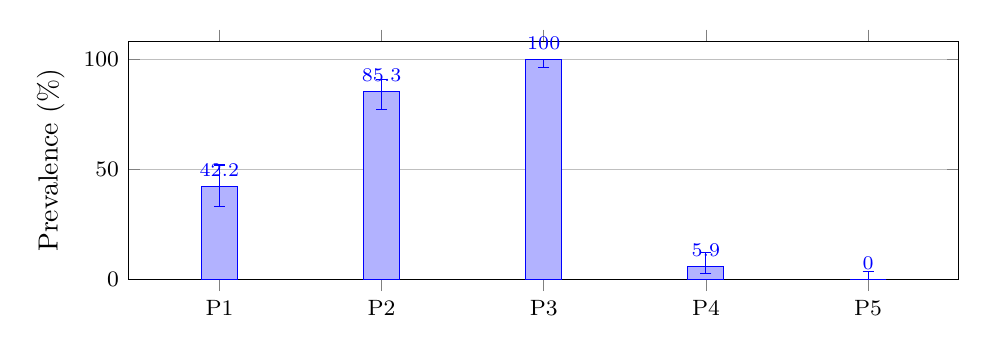
\begin{tikzpicture}
\begin{axis}[
  ybar, bar width=13pt,
  width=\linewidth, height=4.6cm,
  ymin=0, ymax=108, ylabel={Prevalence (\%)},
  symbolic x coords={P1,P2,P3,P4,P5},
  xtick=data, enlarge x limits=0.14,
  nodes near coords, nodes near coords align={vertical},
  every node near coord/.append style={font=\scriptsize},
  ymajorgrids, tick label style={font=\footnotesize},
]
% asymmetric explicit errors:  += (0, upper)  -= (0, lower)
\addplot+[error bars/.cd, y dir=both, y explicit]
coordinates {
  (P1,42.2)  += (0,9.7)  -= (0,9.2)
  (P2,85.3)  += (0,5.6)  -= (0,8.2)
  (P3,100.0) += (0,0.0)  -= (0,3.6)
  (P4,5.9)   += (0,6.3)  -= (0,3.2)
  (P5,0.0)   += (0,3.6)  -= (0,0.0)
};
\end{axis}
\end{tikzpicture}
\caption{Prevalence of cited verification weaknesses across 102 distinct
JWT-validating configurations, with Wilson 95\% confidence intervals.
P1 unbound audience; P2 no required claims; P3 no algorithm pinning \emph{in
configuration} (library-default caveat, \S\ref{sec:results}); P4 multi-issuer
(descriptive); P5 clock skew $>5$\,min. \textbf{Preliminary} (small $N$, no human
labels); see \S\ref{sec:limitations}.}
\label{fig:prevalence}
\end{figure}

\noindent\textbf{Drift (RQ: how contracts change over time).}
Longitudinal analysis over commit history is future work. Today we validate the
drift \emph{classifier} on a 1{,}226-pair synthetic corpus at 100\% recall / 0\%
FPR, with mutation testing (24 mutants, 100\% killed) and a held-out adversarial
set at Youden 0.75. \gate{Drift in the wild, over real commit histories, is left to
the full study.}

\section{Limitations and threats to validity}\label{sec:limitations}
\textbf{Static discovery sees configuration, not the running verifier;} where true
behaviour diverges from config and library defaults, only live probing (out of
scope here) would catch it. \textbf{Templating:} $\approx$17\% of corpus files are
Helm-templated and $\approx$2\% carry kustomize/variable markers, so roughly one in
five configurations is under-resolved without rendering. \textbf{Selection bias:}
public configuration skews to samples, demos, and OSS and is not representative of
private enterprise deployments; this must be stated, not hidden. \textbf{Proxy
oracles:} \S\ref{sec:validation}'s recall/precision are automated approximations
pending human labels. \textbf{Ethics:} we use only public configuration, read
only; we do not probe third-party live endpoints and handle no real tokens;
identifiable high-severity findings follow responsible disclosure.

\section{Related work}\label{sec:related}
\textbf{JWT/OIDC attacks.} Individual verification flaws (\texttt{alg=none}, RS/HS
key confusion, \texttt{jku}/\texttt{kid} injection) are well
documented~\cite{mclean2015jwt,portswigger-jwt}, and OAuth itself has been formally
analysed~\cite{fett2016oauth}. These establish \emph{which} misconfigurations
matter; our contribution is a different one: a \emph{population-scale} view of the
derived contract and its drift, grounded in the same normative
sources~\cite{rfc8725,rfc8707,rfc9728,rfc8693}.
\textbf{IaC/config scanners} (Checkov, KICS, Semgrep~\cite{checkov,kics,semgrep})
pattern-match rules over configuration; we instead \emph{derive} an
attributable auth contract and measure its properties, and our negative control
targets exactly the precision failure pattern-matching is prone to.
\textbf{Contract testing} (Pact~\cite{pact}) borrows the ``contract'' framing but
targets API shape, not auth verification.
\textbf{Measurement studies} of misconfiguration are our methodological template
(pre-registered inclusion, confidence intervals, released artifacts).
\textbf{Agent authorization}~\cite{owaspllm} is a related, fast-moving area treated
in depth by a separate systematization.

\section{A research agenda (vision)}\label{sec:vision}
Beyond the present preliminary measurement, we see a program: (i) scale to a
representative corpus and report prevalence with tight intervals and a
hand-validated extractor; (ii) characterise \emph{drift} longitudinally: do auth
contracts widen more than they narrow, and are widenings tied to reviewable
events?; (iii) quantify the static-vs-runtime frontier: what fraction of
weaknesses are decidable from configuration versus require probing; and
(iv) extend the same instrument to the agent/MCP frontier. This paper contributes
the method, the validated instrument, and the honest baseline that make the
program tractable.

\section{Conclusion}
Authorization correctness is a property of what is running, not of what is written,
and it drifts. We make the implicit token-auth contract explicit, measurable, and
validated with a methodology that is honest about its own limits. The preliminary
measurement and the released instrument are a step toward understanding
auth-verification hygiene at scale.

\section*{Ethics considerations}\label{sec:ethics}
This study measures only \emph{public} configuration, fetched read-only at pinned
commits, and never probes third-party live endpoints or handles real tokens; the
attack surface it characterises is exercised only against local, self-owned
negative-control fixtures. We report \emph{population} prevalence, never a verdict
on any single project, and we name no project as insecure. For any identifiable,
high-severity finding tied to a specific owner we follow coordinated responsible
disclosure before publication, allowing reasonable remediation time. The corpus
respects source licences (recorded per artifact) and robots/rate-limit norms of the
hosting platform. We see no human-subjects concerns; no personal data is collected.

\section*{Open science}\label{sec:openscience}
In keeping with open-science expectations, we release the discovery instrument, the
measurement harness (prevalence with Wilson CIs), the kind-aware validator, the
non-circular negative-control precision test, the analysis scripts, and the corpus
\emph{manifest} (repository + commit SHA + licence per artifact) so the measurement
is reproducible from public sources. \gate{At camera-ready we will add a DOI-pinned
archival snapshot and, where the venue offers it, Artifact-Evaluation ``Available'' and
``Reproduced'' badges.}

\section*{Artifact availability}\label{sec:artifact}
The instrument, harness, validator, negative-control test, and corpus manifest are
open source under the MIT licence. \gate{The archival DOI will be added at
camera-ready.}
. Every unfinished number is wrapped in \gate{...}.
% Submission vs. working-copy rendering. Default: submission (clean prose). A
% wrapper can predefine \submissionfalse before % Shared body for the Paper A measurement study. Class-agnostic: the per-venue
% main.tex sets \documentclass, title, authors, and \begin{document}, then
% % Shared body for the Paper A measurement study. Class-agnostic: the per-venue
% main.tex sets \documentclass, title, authors, and \begin{document}, then
% \input{../common/body}. Every unfinished number is wrapped in \gate{...}.
% Submission vs. working-copy rendering. Default: submission (clean prose). A
% wrapper can predefine \submissionfalse before \input{../common/body} to bring
% back the loud [PENDING]/[NOTE] markers for internal tracking.
\ifdefined\ifsubmission\else\expandafter\newif\csname ifsubmission\endcsname\submissiontrue\fi
% \gate{...}: forward-looking text. Submission -> plain prose; draft -> [PENDING].
% Content is written to read as a finished future-work sentence either way.
\providecommand{\gate}[1]{\ifsubmission #1\else \textbf{[PENDING: #1]}\fi}
% \draftonly{...}: internal note. Submission -> nothing; draft -> [NOTE].
\providecommand{\draftonly}[1]{\ifsubmission\else \textbf{[NOTE: #1]}\fi}
% Let TeX relax line breaking on paragraphs with long unbreakable \texttt{} kind
% names (RequestAuthentication, AuthorizationPolicy) instead of overrunning the
% margin. Class-agnostic; applies under every venue wrapper.
\emergencystretch=3em

\begin{abstract}
Whether a service accepts a bearer token comes down to configuration, not code:
which issuers it trusts, which audiences it binds to, which algorithms it allows,
and which claims it requires. These settings are spread across service meshes,
proxies, and identity providers, they are rarely written down in one place, and a
single change (a rotated key, a widened audience, a dropped claim) silently turns
valid users away or starts admitting tokens that should be refused. We call this
configuration a service's implicit \emph{authorization contract}, and we think it
should be measured directly rather than assumed. We give a method that derives the
contract from deployment configuration and run it over 428 public repositories. In a
first sample of 102 JWT-validating configurations, none pinned a signing algorithm
in configuration (100\%, leaving it to the verifying library's default), 85.3\%
required no claims, and 42.2\% left the token audience unbound, all with Wilson
95\% confidence intervals. Because a measurement is only as good as its extractor,
we validate it two ways and state each method's limits: a kind-aware oracle for
recall (issuers 89.6\%, audiences 99.0\%), and a negative control for precision that
plants values a correct tool must ignore. We release the tool, the corpus manifest,
and the analysis. These numbers are preliminary and from a small sample; the paper
sets out the agenda a full study needs: scale, drift over time, and the line between
what configuration reveals and what only runtime can.
\draftonly{hand-labelled validation and scaled-corpus results before a full-paper
submission; this Vision draft leads with the agenda.}
\end{abstract}

\section{Introduction}
An engineer rotates a signing key on a Friday. No code changes; every test passes.
By Monday a downstream service is rejecting every valid user, because its verifier
cached the retired key longer than anyone realised. The same week, elsewhere, a
verifier quietly begins accepting a second audience nobody intended. Neither
failure lives in the code, and neither would be caught by reading it: both live in
the \emph{configuration} that actually decides whether a bearer token is accepted.

That configuration is an implicit specification: the issuers a verifier trusts,
the audiences it binds to, the algorithms it allows, the claims it requires, and
the JWKS behaviour of the library beneath it. We call it the \emph{authorization
contract}. It is spread across service meshes, proxies, identity providers, and
library defaults, it is almost never centralised, and it \emph{drifts}: a rotated
key, a widened audience, or a dropped claim turns valid users away (an outage) or
admits tokens that should be refused (a silent regression). As autonomous agents
begin carrying OAuth/MCP tokens on a user's behalf, the same contract now governs a
faster-moving, higher-stakes surface.

This contract is where auth correctness actually lives, and yet almost nobody
measures it. Two kinds of tooling exist, and neither answers ``what does the
deployed auth contract look like, at scale, and how healthy is it?'' Static code
scanners reason about source, not about which \emph{running} verifier trusts which
issuer. Gateways and identity providers are the thing being configured, so they
cannot tell you whether that configuration is healthy. We think the authorization
contract should be something you can measure, and this paper is the first step
toward measuring it.

\noindent\textbf{Contributions.}
(i) A way of treating the authorization contract as something you can derive,
version, and measure, and a method to derive it from heterogeneous deployment
configuration with per-field provenance (\S\ref{sec:method}).
(ii) A preliminary measurement of how common concrete, RFC-cited weaknesses are
across 428 public repositories, with confidence intervals (\S\ref{sec:results}).
(iii) A validation methodology that is honest about its own limits: a kind-aware
oracle for recall and a non-circular negative control for precision, each with its
failure mode stated (\S\ref{sec:validation}).
(iv) A released instrument, corpus manifest, and analysis (\S\ref{sec:artifact}),
and a research agenda (scale, drift, and the static/runtime frontier,
\S\ref{sec:vision}) that a full study completes.

\noindent This is a vision-and-first-step paper by design: we contribute the
framing, a validated instrument, and an honest baseline, and we set the agenda we
think the community should pursue. \S\ref{sec:limitations} is open about what the
preliminary measurement does not yet establish.

\section{Background}\label{sec:background}
A JWT verifier is defined by: the \emph{issuers} it trusts, the \emph{audiences}
it binds tokens to (RFC~8707, RFC~9728), the signing \emph{algorithms} it permits
(RFC~8725~\S3.1), the \emph{claims} it requires (RFC~8725~\S3.9), and its
JWKS-fetch/cache behaviour. Agent authorization adds delegation (RFC~8693 \texttt{act}),
resource binding for MCP servers, scope minimisation, and token lifetime. These
are the fields whose prevalence we measure, each grounded in a normative source.

\section{Deriving authorization contracts}\label{sec:method}
A \emph{consumer} is any entity that validates tokens. We derive consumers from
configuration rather than declarations. Discoverers map each source to consumers:
Istio \texttt{RequestAuthentication} (issuer, audiences, JWKS) and
\texttt{AuthorizationPolicy} (required claims in \texttt{when} conditions); Envoy
JWT filters; Kubernetes workload metadata for stable identity; OIDC/Keycloak
registries. Each extracted field records \emph{provenance}
(\{source, locator, confidence\}), so every measurement is attributable to a line
of configuration. A library-defaults database fills verifier behaviour the config
omits, because the contract includes what the verifier does \emph{by default}.
Consumers are assembled into a content-addressed \texttt{ContractVersion}, enabling
exact-equality change detection and diffing across versions.

\section{Corpus construction}\label{sec:corpus}
We crawl public GitHub read-only for real auth configuration (Istio
\texttt{RequestAuthentication}, Envoy \texttt{jwt\_authn}, Istio claim conditions),
recording repository, blob SHA, and licence for every artifact for reproducibility
and attribution. We fetch public repositories only, cap files per repository to
limit monorepo dominance, and analyse \emph{per repository} so a
\texttt{RequestAuthentication} and its \texttt{AuthorizationPolicy} (usually in
separate files) are resolved together while distinct repositories remain isolated.
Two cleaning steps address representativeness: we exclude tutorial/vendored copies
by path, and we deduplicate identical configurations (a canonical sample pasted
across repositories counts once). The preliminary corpus is 603 files across 428
public repositories, yielding 102 distinct JWT-validating configurations after
cleaning. \gate{A full study will scale the corpus toward $10^3$--$10^4$ services
and report the exact $N$ with confidence intervals and a selection-bias analysis.}

\section{Validation methodology}\label{sec:validation}
Measurement is only as good as the extractor. We validate discovery two ways and
are explicit about what each can and cannot establish.

\noindent\textbf{Recall (kind-aware independent parse).} An independent YAML parse
of each repository yields the declared issuers/audiences/claims; we compare to what
discovery captured, per repository. The independent parser also
\emph{over-declares}: it scrapes \texttt{issuer:} keys and claim-like strings from
non-auth resources (a ConfigMap, an annotation). We therefore measure recall only
against values in \emph{genuine} auth resources (RequestAuthentication /
AuthorizationPolicy / Envoy JWT). Adjudicated recall is issuers 89.6\%, audiences
99.0\%, and claims 82.1\% (scoped to repositories where a JWT consumer exists;
claims declared in repositories whose RequestAuthentication is absent from the
corpus have no consumer to attach to). The adjudication removed 17 parser
over-declarations, which both raises the honest recall and demonstrates the proxy
oracle is itself imperfect.

\noindent\textbf{Precision (non-circular negative control).} An independent-parse
oracle cannot honestly measure precision: it reads the same fields as the
extractor, so captures are almost always a subset and precision $\approx 100\%$
\emph{by construction}. We therefore use a negative control: configurations with
planted distractor values a correct discoverer must ignore: a commented-out
issuer, an \texttt{issuer:}/claim in a non-auth ConfigMap, a claim behind a
non-matching AuthorizationPolicy selector (the real attribution risk), and strings
in annotations. Result: 4 planted, 0 leaked, with real values still captured.

\noindent\textbf{Gold standard.} Both above are automated proxies.
\gate{The definitive precision and recall await a hand-labelled stratified sample,
with each captured value adjudicated as real, correctly attributed, or spurious.}

\section{Preliminary results}\label{sec:results}
\emph{These numbers are preliminary (small N, no human labels) and are not to be
cited as final; they are reported to demonstrate the instrument and to bound the
work remaining.}

\noindent\textbf{Prevalence.} Over 102 distinct JWT-validating configurations
(Wilson 95\% CIs): no algorithm pinning \emph{in configuration} 100\%
[96.4, 100]; no required claims 85.3\% [77.1, 90.9]; unbound audience 42.2\%
[33.0, 51.9]. The algorithm-pinning figure reflects reliance on the verifying
\emph{library's default}, which configuration does not restate. This is a
static-vs-runtime gap, not a 100\% vulnerability rate; we report it as
``not pinned in config.''
\gate{We will re-run these over the scaled, hand-labelled corpus and add a
co-occurrence analysis.}

\input{../common/fig-prevalence}

\noindent\textbf{Drift (RQ: how contracts change over time).}
Longitudinal analysis over commit history is future work. Today we validate the
drift \emph{classifier} on a 1{,}226-pair synthetic corpus at 100\% recall / 0\%
FPR, with mutation testing (24 mutants, 100\% killed) and a held-out adversarial
set at Youden 0.75. \gate{Drift in the wild, over real commit histories, is left to
the full study.}

\section{Limitations and threats to validity}\label{sec:limitations}
\textbf{Static discovery sees configuration, not the running verifier;} where true
behaviour diverges from config and library defaults, only live probing (out of
scope here) would catch it. \textbf{Templating:} $\approx$17\% of corpus files are
Helm-templated and $\approx$2\% carry kustomize/variable markers, so roughly one in
five configurations is under-resolved without rendering. \textbf{Selection bias:}
public configuration skews to samples, demos, and OSS and is not representative of
private enterprise deployments; this must be stated, not hidden. \textbf{Proxy
oracles:} \S\ref{sec:validation}'s recall/precision are automated approximations
pending human labels. \textbf{Ethics:} we use only public configuration, read
only; we do not probe third-party live endpoints and handle no real tokens;
identifiable high-severity findings follow responsible disclosure.

\section{Related work}\label{sec:related}
\textbf{JWT/OIDC attacks.} Individual verification flaws (\texttt{alg=none}, RS/HS
key confusion, \texttt{jku}/\texttt{kid} injection) are well
documented~\cite{mclean2015jwt,portswigger-jwt}, and OAuth itself has been formally
analysed~\cite{fett2016oauth}. These establish \emph{which} misconfigurations
matter; our contribution is a different one: a \emph{population-scale} view of the
derived contract and its drift, grounded in the same normative
sources~\cite{rfc8725,rfc8707,rfc9728,rfc8693}.
\textbf{IaC/config scanners} (Checkov, KICS, Semgrep~\cite{checkov,kics,semgrep})
pattern-match rules over configuration; we instead \emph{derive} an
attributable auth contract and measure its properties, and our negative control
targets exactly the precision failure pattern-matching is prone to.
\textbf{Contract testing} (Pact~\cite{pact}) borrows the ``contract'' framing but
targets API shape, not auth verification.
\textbf{Measurement studies} of misconfiguration are our methodological template
(pre-registered inclusion, confidence intervals, released artifacts).
\textbf{Agent authorization}~\cite{owaspllm} is a related, fast-moving area treated
in depth by a separate systematization.

\section{A research agenda (vision)}\label{sec:vision}
Beyond the present preliminary measurement, we see a program: (i) scale to a
representative corpus and report prevalence with tight intervals and a
hand-validated extractor; (ii) characterise \emph{drift} longitudinally: do auth
contracts widen more than they narrow, and are widenings tied to reviewable
events?; (iii) quantify the static-vs-runtime frontier: what fraction of
weaknesses are decidable from configuration versus require probing; and
(iv) extend the same instrument to the agent/MCP frontier. This paper contributes
the method, the validated instrument, and the honest baseline that make the
program tractable.

\section{Conclusion}
Authorization correctness is a property of what is running, not of what is written,
and it drifts. We make the implicit token-auth contract explicit, measurable, and
validated with a methodology that is honest about its own limits. The preliminary
measurement and the released instrument are a step toward understanding
auth-verification hygiene at scale.

\section*{Ethics considerations}\label{sec:ethics}
This study measures only \emph{public} configuration, fetched read-only at pinned
commits, and never probes third-party live endpoints or handles real tokens; the
attack surface it characterises is exercised only against local, self-owned
negative-control fixtures. We report \emph{population} prevalence, never a verdict
on any single project, and we name no project as insecure. For any identifiable,
high-severity finding tied to a specific owner we follow coordinated responsible
disclosure before publication, allowing reasonable remediation time. The corpus
respects source licences (recorded per artifact) and robots/rate-limit norms of the
hosting platform. We see no human-subjects concerns; no personal data is collected.

\section*{Open science}\label{sec:openscience}
In keeping with open-science expectations, we release the discovery instrument, the
measurement harness (prevalence with Wilson CIs), the kind-aware validator, the
non-circular negative-control precision test, the analysis scripts, and the corpus
\emph{manifest} (repository + commit SHA + licence per artifact) so the measurement
is reproducible from public sources. \gate{At camera-ready we will add a DOI-pinned
archival snapshot and, where the venue offers it, Artifact-Evaluation ``Available'' and
``Reproduced'' badges.}

\section*{Artifact availability}\label{sec:artifact}
The instrument, harness, validator, negative-control test, and corpus manifest are
open source under the MIT licence. \gate{The archival DOI will be added at
camera-ready.}
. Every unfinished number is wrapped in \gate{...}.
% Submission vs. working-copy rendering. Default: submission (clean prose). A
% wrapper can predefine \submissionfalse before % Shared body for the Paper A measurement study. Class-agnostic: the per-venue
% main.tex sets \documentclass, title, authors, and \begin{document}, then
% \input{../common/body}. Every unfinished number is wrapped in \gate{...}.
% Submission vs. working-copy rendering. Default: submission (clean prose). A
% wrapper can predefine \submissionfalse before \input{../common/body} to bring
% back the loud [PENDING]/[NOTE] markers for internal tracking.
\ifdefined\ifsubmission\else\expandafter\newif\csname ifsubmission\endcsname\submissiontrue\fi
% \gate{...}: forward-looking text. Submission -> plain prose; draft -> [PENDING].
% Content is written to read as a finished future-work sentence either way.
\providecommand{\gate}[1]{\ifsubmission #1\else \textbf{[PENDING: #1]}\fi}
% \draftonly{...}: internal note. Submission -> nothing; draft -> [NOTE].
\providecommand{\draftonly}[1]{\ifsubmission\else \textbf{[NOTE: #1]}\fi}
% Let TeX relax line breaking on paragraphs with long unbreakable \texttt{} kind
% names (RequestAuthentication, AuthorizationPolicy) instead of overrunning the
% margin. Class-agnostic; applies under every venue wrapper.
\emergencystretch=3em

\begin{abstract}
Whether a service accepts a bearer token comes down to configuration, not code:
which issuers it trusts, which audiences it binds to, which algorithms it allows,
and which claims it requires. These settings are spread across service meshes,
proxies, and identity providers, they are rarely written down in one place, and a
single change (a rotated key, a widened audience, a dropped claim) silently turns
valid users away or starts admitting tokens that should be refused. We call this
configuration a service's implicit \emph{authorization contract}, and we think it
should be measured directly rather than assumed. We give a method that derives the
contract from deployment configuration and run it over 428 public repositories. In a
first sample of 102 JWT-validating configurations, none pinned a signing algorithm
in configuration (100\%, leaving it to the verifying library's default), 85.3\%
required no claims, and 42.2\% left the token audience unbound, all with Wilson
95\% confidence intervals. Because a measurement is only as good as its extractor,
we validate it two ways and state each method's limits: a kind-aware oracle for
recall (issuers 89.6\%, audiences 99.0\%), and a negative control for precision that
plants values a correct tool must ignore. We release the tool, the corpus manifest,
and the analysis. These numbers are preliminary and from a small sample; the paper
sets out the agenda a full study needs: scale, drift over time, and the line between
what configuration reveals and what only runtime can.
\draftonly{hand-labelled validation and scaled-corpus results before a full-paper
submission; this Vision draft leads with the agenda.}
\end{abstract}

\section{Introduction}
An engineer rotates a signing key on a Friday. No code changes; every test passes.
By Monday a downstream service is rejecting every valid user, because its verifier
cached the retired key longer than anyone realised. The same week, elsewhere, a
verifier quietly begins accepting a second audience nobody intended. Neither
failure lives in the code, and neither would be caught by reading it: both live in
the \emph{configuration} that actually decides whether a bearer token is accepted.

That configuration is an implicit specification: the issuers a verifier trusts,
the audiences it binds to, the algorithms it allows, the claims it requires, and
the JWKS behaviour of the library beneath it. We call it the \emph{authorization
contract}. It is spread across service meshes, proxies, identity providers, and
library defaults, it is almost never centralised, and it \emph{drifts}: a rotated
key, a widened audience, or a dropped claim turns valid users away (an outage) or
admits tokens that should be refused (a silent regression). As autonomous agents
begin carrying OAuth/MCP tokens on a user's behalf, the same contract now governs a
faster-moving, higher-stakes surface.

This contract is where auth correctness actually lives, and yet almost nobody
measures it. Two kinds of tooling exist, and neither answers ``what does the
deployed auth contract look like, at scale, and how healthy is it?'' Static code
scanners reason about source, not about which \emph{running} verifier trusts which
issuer. Gateways and identity providers are the thing being configured, so they
cannot tell you whether that configuration is healthy. We think the authorization
contract should be something you can measure, and this paper is the first step
toward measuring it.

\noindent\textbf{Contributions.}
(i) A way of treating the authorization contract as something you can derive,
version, and measure, and a method to derive it from heterogeneous deployment
configuration with per-field provenance (\S\ref{sec:method}).
(ii) A preliminary measurement of how common concrete, RFC-cited weaknesses are
across 428 public repositories, with confidence intervals (\S\ref{sec:results}).
(iii) A validation methodology that is honest about its own limits: a kind-aware
oracle for recall and a non-circular negative control for precision, each with its
failure mode stated (\S\ref{sec:validation}).
(iv) A released instrument, corpus manifest, and analysis (\S\ref{sec:artifact}),
and a research agenda (scale, drift, and the static/runtime frontier,
\S\ref{sec:vision}) that a full study completes.

\noindent This is a vision-and-first-step paper by design: we contribute the
framing, a validated instrument, and an honest baseline, and we set the agenda we
think the community should pursue. \S\ref{sec:limitations} is open about what the
preliminary measurement does not yet establish.

\section{Background}\label{sec:background}
A JWT verifier is defined by: the \emph{issuers} it trusts, the \emph{audiences}
it binds tokens to (RFC~8707, RFC~9728), the signing \emph{algorithms} it permits
(RFC~8725~\S3.1), the \emph{claims} it requires (RFC~8725~\S3.9), and its
JWKS-fetch/cache behaviour. Agent authorization adds delegation (RFC~8693 \texttt{act}),
resource binding for MCP servers, scope minimisation, and token lifetime. These
are the fields whose prevalence we measure, each grounded in a normative source.

\section{Deriving authorization contracts}\label{sec:method}
A \emph{consumer} is any entity that validates tokens. We derive consumers from
configuration rather than declarations. Discoverers map each source to consumers:
Istio \texttt{RequestAuthentication} (issuer, audiences, JWKS) and
\texttt{AuthorizationPolicy} (required claims in \texttt{when} conditions); Envoy
JWT filters; Kubernetes workload metadata for stable identity; OIDC/Keycloak
registries. Each extracted field records \emph{provenance}
(\{source, locator, confidence\}), so every measurement is attributable to a line
of configuration. A library-defaults database fills verifier behaviour the config
omits, because the contract includes what the verifier does \emph{by default}.
Consumers are assembled into a content-addressed \texttt{ContractVersion}, enabling
exact-equality change detection and diffing across versions.

\section{Corpus construction}\label{sec:corpus}
We crawl public GitHub read-only for real auth configuration (Istio
\texttt{RequestAuthentication}, Envoy \texttt{jwt\_authn}, Istio claim conditions),
recording repository, blob SHA, and licence for every artifact for reproducibility
and attribution. We fetch public repositories only, cap files per repository to
limit monorepo dominance, and analyse \emph{per repository} so a
\texttt{RequestAuthentication} and its \texttt{AuthorizationPolicy} (usually in
separate files) are resolved together while distinct repositories remain isolated.
Two cleaning steps address representativeness: we exclude tutorial/vendored copies
by path, and we deduplicate identical configurations (a canonical sample pasted
across repositories counts once). The preliminary corpus is 603 files across 428
public repositories, yielding 102 distinct JWT-validating configurations after
cleaning. \gate{A full study will scale the corpus toward $10^3$--$10^4$ services
and report the exact $N$ with confidence intervals and a selection-bias analysis.}

\section{Validation methodology}\label{sec:validation}
Measurement is only as good as the extractor. We validate discovery two ways and
are explicit about what each can and cannot establish.

\noindent\textbf{Recall (kind-aware independent parse).} An independent YAML parse
of each repository yields the declared issuers/audiences/claims; we compare to what
discovery captured, per repository. The independent parser also
\emph{over-declares}: it scrapes \texttt{issuer:} keys and claim-like strings from
non-auth resources (a ConfigMap, an annotation). We therefore measure recall only
against values in \emph{genuine} auth resources (RequestAuthentication /
AuthorizationPolicy / Envoy JWT). Adjudicated recall is issuers 89.6\%, audiences
99.0\%, and claims 82.1\% (scoped to repositories where a JWT consumer exists;
claims declared in repositories whose RequestAuthentication is absent from the
corpus have no consumer to attach to). The adjudication removed 17 parser
over-declarations, which both raises the honest recall and demonstrates the proxy
oracle is itself imperfect.

\noindent\textbf{Precision (non-circular negative control).} An independent-parse
oracle cannot honestly measure precision: it reads the same fields as the
extractor, so captures are almost always a subset and precision $\approx 100\%$
\emph{by construction}. We therefore use a negative control: configurations with
planted distractor values a correct discoverer must ignore: a commented-out
issuer, an \texttt{issuer:}/claim in a non-auth ConfigMap, a claim behind a
non-matching AuthorizationPolicy selector (the real attribution risk), and strings
in annotations. Result: 4 planted, 0 leaked, with real values still captured.

\noindent\textbf{Gold standard.} Both above are automated proxies.
\gate{The definitive precision and recall await a hand-labelled stratified sample,
with each captured value adjudicated as real, correctly attributed, or spurious.}

\section{Preliminary results}\label{sec:results}
\emph{These numbers are preliminary (small N, no human labels) and are not to be
cited as final; they are reported to demonstrate the instrument and to bound the
work remaining.}

\noindent\textbf{Prevalence.} Over 102 distinct JWT-validating configurations
(Wilson 95\% CIs): no algorithm pinning \emph{in configuration} 100\%
[96.4, 100]; no required claims 85.3\% [77.1, 90.9]; unbound audience 42.2\%
[33.0, 51.9]. The algorithm-pinning figure reflects reliance on the verifying
\emph{library's default}, which configuration does not restate. This is a
static-vs-runtime gap, not a 100\% vulnerability rate; we report it as
``not pinned in config.''
\gate{We will re-run these over the scaled, hand-labelled corpus and add a
co-occurrence analysis.}

\input{../common/fig-prevalence}

\noindent\textbf{Drift (RQ: how contracts change over time).}
Longitudinal analysis over commit history is future work. Today we validate the
drift \emph{classifier} on a 1{,}226-pair synthetic corpus at 100\% recall / 0\%
FPR, with mutation testing (24 mutants, 100\% killed) and a held-out adversarial
set at Youden 0.75. \gate{Drift in the wild, over real commit histories, is left to
the full study.}

\section{Limitations and threats to validity}\label{sec:limitations}
\textbf{Static discovery sees configuration, not the running verifier;} where true
behaviour diverges from config and library defaults, only live probing (out of
scope here) would catch it. \textbf{Templating:} $\approx$17\% of corpus files are
Helm-templated and $\approx$2\% carry kustomize/variable markers, so roughly one in
five configurations is under-resolved without rendering. \textbf{Selection bias:}
public configuration skews to samples, demos, and OSS and is not representative of
private enterprise deployments; this must be stated, not hidden. \textbf{Proxy
oracles:} \S\ref{sec:validation}'s recall/precision are automated approximations
pending human labels. \textbf{Ethics:} we use only public configuration, read
only; we do not probe third-party live endpoints and handle no real tokens;
identifiable high-severity findings follow responsible disclosure.

\section{Related work}\label{sec:related}
\textbf{JWT/OIDC attacks.} Individual verification flaws (\texttt{alg=none}, RS/HS
key confusion, \texttt{jku}/\texttt{kid} injection) are well
documented~\cite{mclean2015jwt,portswigger-jwt}, and OAuth itself has been formally
analysed~\cite{fett2016oauth}. These establish \emph{which} misconfigurations
matter; our contribution is a different one: a \emph{population-scale} view of the
derived contract and its drift, grounded in the same normative
sources~\cite{rfc8725,rfc8707,rfc9728,rfc8693}.
\textbf{IaC/config scanners} (Checkov, KICS, Semgrep~\cite{checkov,kics,semgrep})
pattern-match rules over configuration; we instead \emph{derive} an
attributable auth contract and measure its properties, and our negative control
targets exactly the precision failure pattern-matching is prone to.
\textbf{Contract testing} (Pact~\cite{pact}) borrows the ``contract'' framing but
targets API shape, not auth verification.
\textbf{Measurement studies} of misconfiguration are our methodological template
(pre-registered inclusion, confidence intervals, released artifacts).
\textbf{Agent authorization}~\cite{owaspllm} is a related, fast-moving area treated
in depth by a separate systematization.

\section{A research agenda (vision)}\label{sec:vision}
Beyond the present preliminary measurement, we see a program: (i) scale to a
representative corpus and report prevalence with tight intervals and a
hand-validated extractor; (ii) characterise \emph{drift} longitudinally: do auth
contracts widen more than they narrow, and are widenings tied to reviewable
events?; (iii) quantify the static-vs-runtime frontier: what fraction of
weaknesses are decidable from configuration versus require probing; and
(iv) extend the same instrument to the agent/MCP frontier. This paper contributes
the method, the validated instrument, and the honest baseline that make the
program tractable.

\section{Conclusion}
Authorization correctness is a property of what is running, not of what is written,
and it drifts. We make the implicit token-auth contract explicit, measurable, and
validated with a methodology that is honest about its own limits. The preliminary
measurement and the released instrument are a step toward understanding
auth-verification hygiene at scale.

\section*{Ethics considerations}\label{sec:ethics}
This study measures only \emph{public} configuration, fetched read-only at pinned
commits, and never probes third-party live endpoints or handles real tokens; the
attack surface it characterises is exercised only against local, self-owned
negative-control fixtures. We report \emph{population} prevalence, never a verdict
on any single project, and we name no project as insecure. For any identifiable,
high-severity finding tied to a specific owner we follow coordinated responsible
disclosure before publication, allowing reasonable remediation time. The corpus
respects source licences (recorded per artifact) and robots/rate-limit norms of the
hosting platform. We see no human-subjects concerns; no personal data is collected.

\section*{Open science}\label{sec:openscience}
In keeping with open-science expectations, we release the discovery instrument, the
measurement harness (prevalence with Wilson CIs), the kind-aware validator, the
non-circular negative-control precision test, the analysis scripts, and the corpus
\emph{manifest} (repository + commit SHA + licence per artifact) so the measurement
is reproducible from public sources. \gate{At camera-ready we will add a DOI-pinned
archival snapshot and, where the venue offers it, Artifact-Evaluation ``Available'' and
``Reproduced'' badges.}

\section*{Artifact availability}\label{sec:artifact}
The instrument, harness, validator, negative-control test, and corpus manifest are
open source under the MIT licence. \gate{The archival DOI will be added at
camera-ready.}
 to bring
% back the loud [PENDING]/[NOTE] markers for internal tracking.
\ifdefined\ifsubmission\else\expandafter\newif\csname ifsubmission\endcsname\submissiontrue\fi
% \gate{...}: forward-looking text. Submission -> plain prose; draft -> [PENDING].
% Content is written to read as a finished future-work sentence either way.
\providecommand{\gate}[1]{\ifsubmission #1\else \textbf{[PENDING: #1]}\fi}
% \draftonly{...}: internal note. Submission -> nothing; draft -> [NOTE].
\providecommand{\draftonly}[1]{\ifsubmission\else \textbf{[NOTE: #1]}\fi}
% Let TeX relax line breaking on paragraphs with long unbreakable \texttt{} kind
% names (RequestAuthentication, AuthorizationPolicy) instead of overrunning the
% margin. Class-agnostic; applies under every venue wrapper.
\emergencystretch=3em

\begin{abstract}
Whether a service accepts a bearer token comes down to configuration, not code:
which issuers it trusts, which audiences it binds to, which algorithms it allows,
and which claims it requires. These settings are spread across service meshes,
proxies, and identity providers, they are rarely written down in one place, and a
single change (a rotated key, a widened audience, a dropped claim) silently turns
valid users away or starts admitting tokens that should be refused. We call this
configuration a service's implicit \emph{authorization contract}, and we think it
should be measured directly rather than assumed. We give a method that derives the
contract from deployment configuration and run it over 428 public repositories. In a
first sample of 102 JWT-validating configurations, none pinned a signing algorithm
in configuration (100\%, leaving it to the verifying library's default), 85.3\%
required no claims, and 42.2\% left the token audience unbound, all with Wilson
95\% confidence intervals. Because a measurement is only as good as its extractor,
we validate it two ways and state each method's limits: a kind-aware oracle for
recall (issuers 89.6\%, audiences 99.0\%), and a negative control for precision that
plants values a correct tool must ignore. We release the tool, the corpus manifest,
and the analysis. These numbers are preliminary and from a small sample; the paper
sets out the agenda a full study needs: scale, drift over time, and the line between
what configuration reveals and what only runtime can.
\draftonly{hand-labelled validation and scaled-corpus results before a full-paper
submission; this Vision draft leads with the agenda.}
\end{abstract}

\section{Introduction}
An engineer rotates a signing key on a Friday. No code changes; every test passes.
By Monday a downstream service is rejecting every valid user, because its verifier
cached the retired key longer than anyone realised. The same week, elsewhere, a
verifier quietly begins accepting a second audience nobody intended. Neither
failure lives in the code, and neither would be caught by reading it: both live in
the \emph{configuration} that actually decides whether a bearer token is accepted.

That configuration is an implicit specification: the issuers a verifier trusts,
the audiences it binds to, the algorithms it allows, the claims it requires, and
the JWKS behaviour of the library beneath it. We call it the \emph{authorization
contract}. It is spread across service meshes, proxies, identity providers, and
library defaults, it is almost never centralised, and it \emph{drifts}: a rotated
key, a widened audience, or a dropped claim turns valid users away (an outage) or
admits tokens that should be refused (a silent regression). As autonomous agents
begin carrying OAuth/MCP tokens on a user's behalf, the same contract now governs a
faster-moving, higher-stakes surface.

This contract is where auth correctness actually lives, and yet almost nobody
measures it. Two kinds of tooling exist, and neither answers ``what does the
deployed auth contract look like, at scale, and how healthy is it?'' Static code
scanners reason about source, not about which \emph{running} verifier trusts which
issuer. Gateways and identity providers are the thing being configured, so they
cannot tell you whether that configuration is healthy. We think the authorization
contract should be something you can measure, and this paper is the first step
toward measuring it.

\noindent\textbf{Contributions.}
(i) A way of treating the authorization contract as something you can derive,
version, and measure, and a method to derive it from heterogeneous deployment
configuration with per-field provenance (\S\ref{sec:method}).
(ii) A preliminary measurement of how common concrete, RFC-cited weaknesses are
across 428 public repositories, with confidence intervals (\S\ref{sec:results}).
(iii) A validation methodology that is honest about its own limits: a kind-aware
oracle for recall and a non-circular negative control for precision, each with its
failure mode stated (\S\ref{sec:validation}).
(iv) A released instrument, corpus manifest, and analysis (\S\ref{sec:artifact}),
and a research agenda (scale, drift, and the static/runtime frontier,
\S\ref{sec:vision}) that a full study completes.

\noindent This is a vision-and-first-step paper by design: we contribute the
framing, a validated instrument, and an honest baseline, and we set the agenda we
think the community should pursue. \S\ref{sec:limitations} is open about what the
preliminary measurement does not yet establish.

\section{Background}\label{sec:background}
A JWT verifier is defined by: the \emph{issuers} it trusts, the \emph{audiences}
it binds tokens to (RFC~8707, RFC~9728), the signing \emph{algorithms} it permits
(RFC~8725~\S3.1), the \emph{claims} it requires (RFC~8725~\S3.9), and its
JWKS-fetch/cache behaviour. Agent authorization adds delegation (RFC~8693 \texttt{act}),
resource binding for MCP servers, scope minimisation, and token lifetime. These
are the fields whose prevalence we measure, each grounded in a normative source.

\section{Deriving authorization contracts}\label{sec:method}
A \emph{consumer} is any entity that validates tokens. We derive consumers from
configuration rather than declarations. Discoverers map each source to consumers:
Istio \texttt{RequestAuthentication} (issuer, audiences, JWKS) and
\texttt{AuthorizationPolicy} (required claims in \texttt{when} conditions); Envoy
JWT filters; Kubernetes workload metadata for stable identity; OIDC/Keycloak
registries. Each extracted field records \emph{provenance}
(\{source, locator, confidence\}), so every measurement is attributable to a line
of configuration. A library-defaults database fills verifier behaviour the config
omits, because the contract includes what the verifier does \emph{by default}.
Consumers are assembled into a content-addressed \texttt{ContractVersion}, enabling
exact-equality change detection and diffing across versions.

\section{Corpus construction}\label{sec:corpus}
We crawl public GitHub read-only for real auth configuration (Istio
\texttt{RequestAuthentication}, Envoy \texttt{jwt\_authn}, Istio claim conditions),
recording repository, blob SHA, and licence for every artifact for reproducibility
and attribution. We fetch public repositories only, cap files per repository to
limit monorepo dominance, and analyse \emph{per repository} so a
\texttt{RequestAuthentication} and its \texttt{AuthorizationPolicy} (usually in
separate files) are resolved together while distinct repositories remain isolated.
Two cleaning steps address representativeness: we exclude tutorial/vendored copies
by path, and we deduplicate identical configurations (a canonical sample pasted
across repositories counts once). The preliminary corpus is 603 files across 428
public repositories, yielding 102 distinct JWT-validating configurations after
cleaning. \gate{A full study will scale the corpus toward $10^3$--$10^4$ services
and report the exact $N$ with confidence intervals and a selection-bias analysis.}

\section{Validation methodology}\label{sec:validation}
Measurement is only as good as the extractor. We validate discovery two ways and
are explicit about what each can and cannot establish.

\noindent\textbf{Recall (kind-aware independent parse).} An independent YAML parse
of each repository yields the declared issuers/audiences/claims; we compare to what
discovery captured, per repository. The independent parser also
\emph{over-declares}: it scrapes \texttt{issuer:} keys and claim-like strings from
non-auth resources (a ConfigMap, an annotation). We therefore measure recall only
against values in \emph{genuine} auth resources (RequestAuthentication /
AuthorizationPolicy / Envoy JWT). Adjudicated recall is issuers 89.6\%, audiences
99.0\%, and claims 82.1\% (scoped to repositories where a JWT consumer exists;
claims declared in repositories whose RequestAuthentication is absent from the
corpus have no consumer to attach to). The adjudication removed 17 parser
over-declarations, which both raises the honest recall and demonstrates the proxy
oracle is itself imperfect.

\noindent\textbf{Precision (non-circular negative control).} An independent-parse
oracle cannot honestly measure precision: it reads the same fields as the
extractor, so captures are almost always a subset and precision $\approx 100\%$
\emph{by construction}. We therefore use a negative control: configurations with
planted distractor values a correct discoverer must ignore: a commented-out
issuer, an \texttt{issuer:}/claim in a non-auth ConfigMap, a claim behind a
non-matching AuthorizationPolicy selector (the real attribution risk), and strings
in annotations. Result: 4 planted, 0 leaked, with real values still captured.

\noindent\textbf{Gold standard.} Both above are automated proxies.
\gate{The definitive precision and recall await a hand-labelled stratified sample,
with each captured value adjudicated as real, correctly attributed, or spurious.}

\section{Preliminary results}\label{sec:results}
\emph{These numbers are preliminary (small N, no human labels) and are not to be
cited as final; they are reported to demonstrate the instrument and to bound the
work remaining.}

\noindent\textbf{Prevalence.} Over 102 distinct JWT-validating configurations
(Wilson 95\% CIs): no algorithm pinning \emph{in configuration} 100\%
[96.4, 100]; no required claims 85.3\% [77.1, 90.9]; unbound audience 42.2\%
[33.0, 51.9]. The algorithm-pinning figure reflects reliance on the verifying
\emph{library's default}, which configuration does not restate. This is a
static-vs-runtime gap, not a 100\% vulnerability rate; we report it as
``not pinned in config.''
\gate{We will re-run these over the scaled, hand-labelled corpus and add a
co-occurrence analysis.}

% Prevalence figure (preliminary, n=102 distinct JWT-validating configs).
% Real values with Wilson 95% CIs (asymmetric). Requires pgfplots in the preamble
% (the wrappers add it). \input this inside the Results section.
\begin{figure}[t]
\centering
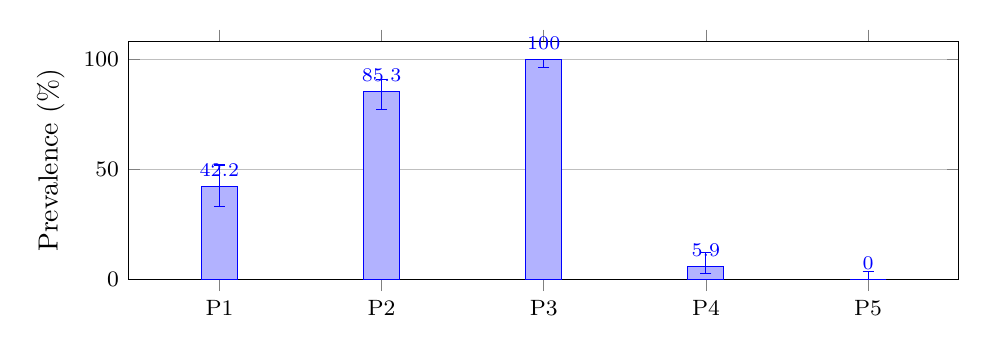
\begin{tikzpicture}
\begin{axis}[
  ybar, bar width=13pt,
  width=\linewidth, height=4.6cm,
  ymin=0, ymax=108, ylabel={Prevalence (\%)},
  symbolic x coords={P1,P2,P3,P4,P5},
  xtick=data, enlarge x limits=0.14,
  nodes near coords, nodes near coords align={vertical},
  every node near coord/.append style={font=\scriptsize},
  ymajorgrids, tick label style={font=\footnotesize},
]
% asymmetric explicit errors:  += (0, upper)  -= (0, lower)
\addplot+[error bars/.cd, y dir=both, y explicit]
coordinates {
  (P1,42.2)  += (0,9.7)  -= (0,9.2)
  (P2,85.3)  += (0,5.6)  -= (0,8.2)
  (P3,100.0) += (0,0.0)  -= (0,3.6)
  (P4,5.9)   += (0,6.3)  -= (0,3.2)
  (P5,0.0)   += (0,3.6)  -= (0,0.0)
};
\end{axis}
\end{tikzpicture}
\caption{Prevalence of cited verification weaknesses across 102 distinct
JWT-validating configurations, with Wilson 95\% confidence intervals.
P1 unbound audience; P2 no required claims; P3 no algorithm pinning \emph{in
configuration} (library-default caveat, \S\ref{sec:results}); P4 multi-issuer
(descriptive); P5 clock skew $>5$\,min. \textbf{Preliminary} (small $N$, no human
labels); see \S\ref{sec:limitations}.}
\label{fig:prevalence}
\end{figure}

\noindent\textbf{Drift (RQ: how contracts change over time).}
Longitudinal analysis over commit history is future work. Today we validate the
drift \emph{classifier} on a 1{,}226-pair synthetic corpus at 100\% recall / 0\%
FPR, with mutation testing (24 mutants, 100\% killed) and a held-out adversarial
set at Youden 0.75. \gate{Drift in the wild, over real commit histories, is left to
the full study.}

\section{Limitations and threats to validity}\label{sec:limitations}
\textbf{Static discovery sees configuration, not the running verifier;} where true
behaviour diverges from config and library defaults, only live probing (out of
scope here) would catch it. \textbf{Templating:} $\approx$17\% of corpus files are
Helm-templated and $\approx$2\% carry kustomize/variable markers, so roughly one in
five configurations is under-resolved without rendering. \textbf{Selection bias:}
public configuration skews to samples, demos, and OSS and is not representative of
private enterprise deployments; this must be stated, not hidden. \textbf{Proxy
oracles:} \S\ref{sec:validation}'s recall/precision are automated approximations
pending human labels. \textbf{Ethics:} we use only public configuration, read
only; we do not probe third-party live endpoints and handle no real tokens;
identifiable high-severity findings follow responsible disclosure.

\section{Related work}\label{sec:related}
\textbf{JWT/OIDC attacks.} Individual verification flaws (\texttt{alg=none}, RS/HS
key confusion, \texttt{jku}/\texttt{kid} injection) are well
documented~\cite{mclean2015jwt,portswigger-jwt}, and OAuth itself has been formally
analysed~\cite{fett2016oauth}. These establish \emph{which} misconfigurations
matter; our contribution is a different one: a \emph{population-scale} view of the
derived contract and its drift, grounded in the same normative
sources~\cite{rfc8725,rfc8707,rfc9728,rfc8693}.
\textbf{IaC/config scanners} (Checkov, KICS, Semgrep~\cite{checkov,kics,semgrep})
pattern-match rules over configuration; we instead \emph{derive} an
attributable auth contract and measure its properties, and our negative control
targets exactly the precision failure pattern-matching is prone to.
\textbf{Contract testing} (Pact~\cite{pact}) borrows the ``contract'' framing but
targets API shape, not auth verification.
\textbf{Measurement studies} of misconfiguration are our methodological template
(pre-registered inclusion, confidence intervals, released artifacts).
\textbf{Agent authorization}~\cite{owaspllm} is a related, fast-moving area treated
in depth by a separate systematization.

\section{A research agenda (vision)}\label{sec:vision}
Beyond the present preliminary measurement, we see a program: (i) scale to a
representative corpus and report prevalence with tight intervals and a
hand-validated extractor; (ii) characterise \emph{drift} longitudinally: do auth
contracts widen more than they narrow, and are widenings tied to reviewable
events?; (iii) quantify the static-vs-runtime frontier: what fraction of
weaknesses are decidable from configuration versus require probing; and
(iv) extend the same instrument to the agent/MCP frontier. This paper contributes
the method, the validated instrument, and the honest baseline that make the
program tractable.

\section{Conclusion}
Authorization correctness is a property of what is running, not of what is written,
and it drifts. We make the implicit token-auth contract explicit, measurable, and
validated with a methodology that is honest about its own limits. The preliminary
measurement and the released instrument are a step toward understanding
auth-verification hygiene at scale.

\section*{Ethics considerations}\label{sec:ethics}
This study measures only \emph{public} configuration, fetched read-only at pinned
commits, and never probes third-party live endpoints or handles real tokens; the
attack surface it characterises is exercised only against local, self-owned
negative-control fixtures. We report \emph{population} prevalence, never a verdict
on any single project, and we name no project as insecure. For any identifiable,
high-severity finding tied to a specific owner we follow coordinated responsible
disclosure before publication, allowing reasonable remediation time. The corpus
respects source licences (recorded per artifact) and robots/rate-limit norms of the
hosting platform. We see no human-subjects concerns; no personal data is collected.

\section*{Open science}\label{sec:openscience}
In keeping with open-science expectations, we release the discovery instrument, the
measurement harness (prevalence with Wilson CIs), the kind-aware validator, the
non-circular negative-control precision test, the analysis scripts, and the corpus
\emph{manifest} (repository + commit SHA + licence per artifact) so the measurement
is reproducible from public sources. \gate{At camera-ready we will add a DOI-pinned
archival snapshot and, where the venue offers it, Artifact-Evaluation ``Available'' and
``Reproduced'' badges.}

\section*{Artifact availability}\label{sec:artifact}
The instrument, harness, validator, negative-control test, and corpus manifest are
open source under the MIT licence. \gate{The archival DOI will be added at
camera-ready.}
 to bring
% back the loud [PENDING]/[NOTE] markers for internal tracking.
\ifdefined\ifsubmission\else\expandafter\newif\csname ifsubmission\endcsname\submissiontrue\fi
% \gate{...}: forward-looking text. Submission -> plain prose; draft -> [PENDING].
% Content is written to read as a finished future-work sentence either way.
\providecommand{\gate}[1]{\ifsubmission #1\else \textbf{[PENDING: #1]}\fi}
% \draftonly{...}: internal note. Submission -> nothing; draft -> [NOTE].
\providecommand{\draftonly}[1]{\ifsubmission\else \textbf{[NOTE: #1]}\fi}
% Let TeX relax line breaking on paragraphs with long unbreakable \texttt{} kind
% names (RequestAuthentication, AuthorizationPolicy) instead of overrunning the
% margin. Class-agnostic; applies under every venue wrapper.
\emergencystretch=3em

\begin{abstract}
Whether a service accepts a bearer token comes down to configuration, not code:
which issuers it trusts, which audiences it binds to, which algorithms it allows,
and which claims it requires. These settings are spread across service meshes,
proxies, and identity providers, they are rarely written down in one place, and a
single change (a rotated key, a widened audience, a dropped claim) silently turns
valid users away or starts admitting tokens that should be refused. We call this
configuration a service's implicit \emph{authorization contract}, and we think it
should be measured directly rather than assumed. We give a method that derives the
contract from deployment configuration and run it over 428 public repositories. In a
first sample of 102 JWT-validating configurations, none pinned a signing algorithm
in configuration (100\%, leaving it to the verifying library's default), 85.3\%
required no claims, and 42.2\% left the token audience unbound, all with Wilson
95\% confidence intervals. Because a measurement is only as good as its extractor,
we validate it two ways and state each method's limits: a kind-aware oracle for
recall (issuers 89.6\%, audiences 99.0\%), and a negative control for precision that
plants values a correct tool must ignore. We release the tool, the corpus manifest,
and the analysis. These numbers are preliminary and from a small sample; the paper
sets out the agenda a full study needs: scale, drift over time, and the line between
what configuration reveals and what only runtime can.
\draftonly{hand-labelled validation and scaled-corpus results before a full-paper
submission; this Vision draft leads with the agenda.}
\end{abstract}

\section{Introduction}
An engineer rotates a signing key on a Friday. No code changes; every test passes.
By Monday a downstream service is rejecting every valid user, because its verifier
cached the retired key longer than anyone realised. The same week, elsewhere, a
verifier quietly begins accepting a second audience nobody intended. Neither
failure lives in the code, and neither would be caught by reading it: both live in
the \emph{configuration} that actually decides whether a bearer token is accepted.

That configuration is an implicit specification: the issuers a verifier trusts,
the audiences it binds to, the algorithms it allows, the claims it requires, and
the JWKS behaviour of the library beneath it. We call it the \emph{authorization
contract}. It is spread across service meshes, proxies, identity providers, and
library defaults, it is almost never centralised, and it \emph{drifts}: a rotated
key, a widened audience, or a dropped claim turns valid users away (an outage) or
admits tokens that should be refused (a silent regression). As autonomous agents
begin carrying OAuth/MCP tokens on a user's behalf, the same contract now governs a
faster-moving, higher-stakes surface.

This contract is where auth correctness actually lives, and yet almost nobody
measures it. Two kinds of tooling exist, and neither answers ``what does the
deployed auth contract look like, at scale, and how healthy is it?'' Static code
scanners reason about source, not about which \emph{running} verifier trusts which
issuer. Gateways and identity providers are the thing being configured, so they
cannot tell you whether that configuration is healthy. We think the authorization
contract should be something you can measure, and this paper is the first step
toward measuring it.

\noindent\textbf{Contributions.}
(i) A way of treating the authorization contract as something you can derive,
version, and measure, and a method to derive it from heterogeneous deployment
configuration with per-field provenance (\S\ref{sec:method}).
(ii) A preliminary measurement of how common concrete, RFC-cited weaknesses are
across 428 public repositories, with confidence intervals (\S\ref{sec:results}).
(iii) A validation methodology that is honest about its own limits: a kind-aware
oracle for recall and a non-circular negative control for precision, each with its
failure mode stated (\S\ref{sec:validation}).
(iv) A released instrument, corpus manifest, and analysis (\S\ref{sec:artifact}),
and a research agenda (scale, drift, and the static/runtime frontier,
\S\ref{sec:vision}) that a full study completes.

\noindent This is a vision-and-first-step paper by design: we contribute the
framing, a validated instrument, and an honest baseline, and we set the agenda we
think the community should pursue. \S\ref{sec:limitations} is open about what the
preliminary measurement does not yet establish.

\section{Background}\label{sec:background}
A JWT verifier is defined by: the \emph{issuers} it trusts, the \emph{audiences}
it binds tokens to (RFC~8707, RFC~9728), the signing \emph{algorithms} it permits
(RFC~8725~\S3.1), the \emph{claims} it requires (RFC~8725~\S3.9), and its
JWKS-fetch/cache behaviour. Agent authorization adds delegation (RFC~8693 \texttt{act}),
resource binding for MCP servers, scope minimisation, and token lifetime. These
are the fields whose prevalence we measure, each grounded in a normative source.

\section{Deriving authorization contracts}\label{sec:method}
A \emph{consumer} is any entity that validates tokens. We derive consumers from
configuration rather than declarations. Discoverers map each source to consumers:
Istio \texttt{RequestAuthentication} (issuer, audiences, JWKS) and
\texttt{AuthorizationPolicy} (required claims in \texttt{when} conditions); Envoy
JWT filters; Kubernetes workload metadata for stable identity; OIDC/Keycloak
registries. Each extracted field records \emph{provenance}
(\{source, locator, confidence\}), so every measurement is attributable to a line
of configuration. A library-defaults database fills verifier behaviour the config
omits, because the contract includes what the verifier does \emph{by default}.
Consumers are assembled into a content-addressed \texttt{ContractVersion}, enabling
exact-equality change detection and diffing across versions.

\section{Corpus construction}\label{sec:corpus}
We crawl public GitHub read-only for real auth configuration (Istio
\texttt{RequestAuthentication}, Envoy \texttt{jwt\_authn}, Istio claim conditions),
recording repository, blob SHA, and licence for every artifact for reproducibility
and attribution. We fetch public repositories only, cap files per repository to
limit monorepo dominance, and analyse \emph{per repository} so a
\texttt{RequestAuthentication} and its \texttt{AuthorizationPolicy} (usually in
separate files) are resolved together while distinct repositories remain isolated.
Two cleaning steps address representativeness: we exclude tutorial/vendored copies
by path, and we deduplicate identical configurations (a canonical sample pasted
across repositories counts once). The preliminary corpus is 603 files across 428
public repositories, yielding 102 distinct JWT-validating configurations after
cleaning. \gate{A full study will scale the corpus toward $10^3$--$10^4$ services
and report the exact $N$ with confidence intervals and a selection-bias analysis.}

\section{Validation methodology}\label{sec:validation}
Measurement is only as good as the extractor. We validate discovery two ways and
are explicit about what each can and cannot establish.

\noindent\textbf{Recall (kind-aware independent parse).} An independent YAML parse
of each repository yields the declared issuers/audiences/claims; we compare to what
discovery captured, per repository. The independent parser also
\emph{over-declares}: it scrapes \texttt{issuer:} keys and claim-like strings from
non-auth resources (a ConfigMap, an annotation). We therefore measure recall only
against values in \emph{genuine} auth resources (RequestAuthentication /
AuthorizationPolicy / Envoy JWT). Adjudicated recall is issuers 89.6\%, audiences
99.0\%, and claims 82.1\% (scoped to repositories where a JWT consumer exists;
claims declared in repositories whose RequestAuthentication is absent from the
corpus have no consumer to attach to). The adjudication removed 17 parser
over-declarations, which both raises the honest recall and demonstrates the proxy
oracle is itself imperfect.

\noindent\textbf{Precision (non-circular negative control).} An independent-parse
oracle cannot honestly measure precision: it reads the same fields as the
extractor, so captures are almost always a subset and precision $\approx 100\%$
\emph{by construction}. We therefore use a negative control: configurations with
planted distractor values a correct discoverer must ignore: a commented-out
issuer, an \texttt{issuer:}/claim in a non-auth ConfigMap, a claim behind a
non-matching AuthorizationPolicy selector (the real attribution risk), and strings
in annotations. Result: 4 planted, 0 leaked, with real values still captured.

\noindent\textbf{Gold standard.} Both above are automated proxies.
\gate{The definitive precision and recall await a hand-labelled stratified sample,
with each captured value adjudicated as real, correctly attributed, or spurious.}

\section{Preliminary results}\label{sec:results}
\emph{These numbers are preliminary (small N, no human labels) and are not to be
cited as final; they are reported to demonstrate the instrument and to bound the
work remaining.}

\noindent\textbf{Prevalence.} Over 102 distinct JWT-validating configurations
(Wilson 95\% CIs): no algorithm pinning \emph{in configuration} 100\%
[96.4, 100]; no required claims 85.3\% [77.1, 90.9]; unbound audience 42.2\%
[33.0, 51.9]. The algorithm-pinning figure reflects reliance on the verifying
\emph{library's default}, which configuration does not restate. This is a
static-vs-runtime gap, not a 100\% vulnerability rate; we report it as
``not pinned in config.''
\gate{We will re-run these over the scaled, hand-labelled corpus and add a
co-occurrence analysis.}

% Prevalence figure (preliminary, n=102 distinct JWT-validating configs).
% Real values with Wilson 95% CIs (asymmetric). Requires pgfplots in the preamble
% (the wrappers add it). \input this inside the Results section.
\begin{figure}[t]
\centering
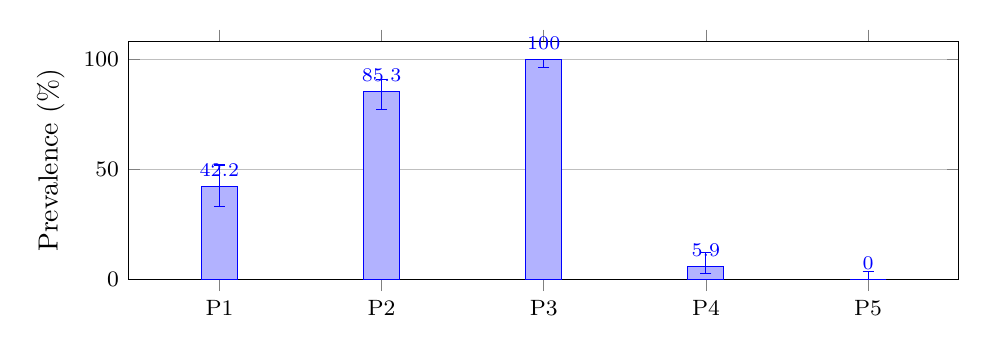
\begin{tikzpicture}
\begin{axis}[
  ybar, bar width=13pt,
  width=\linewidth, height=4.6cm,
  ymin=0, ymax=108, ylabel={Prevalence (\%)},
  symbolic x coords={P1,P2,P3,P4,P5},
  xtick=data, enlarge x limits=0.14,
  nodes near coords, nodes near coords align={vertical},
  every node near coord/.append style={font=\scriptsize},
  ymajorgrids, tick label style={font=\footnotesize},
]
% asymmetric explicit errors:  += (0, upper)  -= (0, lower)
\addplot+[error bars/.cd, y dir=both, y explicit]
coordinates {
  (P1,42.2)  += (0,9.7)  -= (0,9.2)
  (P2,85.3)  += (0,5.6)  -= (0,8.2)
  (P3,100.0) += (0,0.0)  -= (0,3.6)
  (P4,5.9)   += (0,6.3)  -= (0,3.2)
  (P5,0.0)   += (0,3.6)  -= (0,0.0)
};
\end{axis}
\end{tikzpicture}
\caption{Prevalence of cited verification weaknesses across 102 distinct
JWT-validating configurations, with Wilson 95\% confidence intervals.
P1 unbound audience; P2 no required claims; P3 no algorithm pinning \emph{in
configuration} (library-default caveat, \S\ref{sec:results}); P4 multi-issuer
(descriptive); P5 clock skew $>5$\,min. \textbf{Preliminary} (small $N$, no human
labels); see \S\ref{sec:limitations}.}
\label{fig:prevalence}
\end{figure}

\noindent\textbf{Drift (RQ: how contracts change over time).}
Longitudinal analysis over commit history is future work. Today we validate the
drift \emph{classifier} on a 1{,}226-pair synthetic corpus at 100\% recall / 0\%
FPR, with mutation testing (24 mutants, 100\% killed) and a held-out adversarial
set at Youden 0.75. \gate{Drift in the wild, over real commit histories, is left to
the full study.}

\section{Limitations and threats to validity}\label{sec:limitations}
\textbf{Static discovery sees configuration, not the running verifier;} where true
behaviour diverges from config and library defaults, only live probing (out of
scope here) would catch it. \textbf{Templating:} $\approx$17\% of corpus files are
Helm-templated and $\approx$2\% carry kustomize/variable markers, so roughly one in
five configurations is under-resolved without rendering. \textbf{Selection bias:}
public configuration skews to samples, demos, and OSS and is not representative of
private enterprise deployments; this must be stated, not hidden. \textbf{Proxy
oracles:} \S\ref{sec:validation}'s recall/precision are automated approximations
pending human labels. \textbf{Ethics:} we use only public configuration, read
only; we do not probe third-party live endpoints and handle no real tokens;
identifiable high-severity findings follow responsible disclosure.

\section{Related work}\label{sec:related}
\textbf{JWT/OIDC attacks.} Individual verification flaws (\texttt{alg=none}, RS/HS
key confusion, \texttt{jku}/\texttt{kid} injection) are well
documented~\cite{mclean2015jwt,portswigger-jwt}, and OAuth itself has been formally
analysed~\cite{fett2016oauth}. These establish \emph{which} misconfigurations
matter; our contribution is a different one: a \emph{population-scale} view of the
derived contract and its drift, grounded in the same normative
sources~\cite{rfc8725,rfc8707,rfc9728,rfc8693}.
\textbf{IaC/config scanners} (Checkov, KICS, Semgrep~\cite{checkov,kics,semgrep})
pattern-match rules over configuration; we instead \emph{derive} an
attributable auth contract and measure its properties, and our negative control
targets exactly the precision failure pattern-matching is prone to.
\textbf{Contract testing} (Pact~\cite{pact}) borrows the ``contract'' framing but
targets API shape, not auth verification.
\textbf{Measurement studies} of misconfiguration are our methodological template
(pre-registered inclusion, confidence intervals, released artifacts).
\textbf{Agent authorization}~\cite{owaspllm} is a related, fast-moving area treated
in depth by a separate systematization.

\section{A research agenda (vision)}\label{sec:vision}
Beyond the present preliminary measurement, we see a program: (i) scale to a
representative corpus and report prevalence with tight intervals and a
hand-validated extractor; (ii) characterise \emph{drift} longitudinally: do auth
contracts widen more than they narrow, and are widenings tied to reviewable
events?; (iii) quantify the static-vs-runtime frontier: what fraction of
weaknesses are decidable from configuration versus require probing; and
(iv) extend the same instrument to the agent/MCP frontier. This paper contributes
the method, the validated instrument, and the honest baseline that make the
program tractable.

\section{Conclusion}
Authorization correctness is a property of what is running, not of what is written,
and it drifts. We make the implicit token-auth contract explicit, measurable, and
validated with a methodology that is honest about its own limits. The preliminary
measurement and the released instrument are a step toward understanding
auth-verification hygiene at scale.

\section*{Ethics considerations}\label{sec:ethics}
This study measures only \emph{public} configuration, fetched read-only at pinned
commits, and never probes third-party live endpoints or handles real tokens; the
attack surface it characterises is exercised only against local, self-owned
negative-control fixtures. We report \emph{population} prevalence, never a verdict
on any single project, and we name no project as insecure. For any identifiable,
high-severity finding tied to a specific owner we follow coordinated responsible
disclosure before publication, allowing reasonable remediation time. The corpus
respects source licences (recorded per artifact) and robots/rate-limit norms of the
hosting platform. We see no human-subjects concerns; no personal data is collected.

\section*{Open science}\label{sec:openscience}
In keeping with open-science expectations, we release the discovery instrument, the
measurement harness (prevalence with Wilson CIs), the kind-aware validator, the
non-circular negative-control precision test, the analysis scripts, and the corpus
\emph{manifest} (repository + commit SHA + licence per artifact) so the measurement
is reproducible from public sources. \gate{At camera-ready we will add a DOI-pinned
archival snapshot and, where the venue offers it, Artifact-Evaluation ``Available'' and
``Reproduced'' badges.}

\section*{Artifact availability}\label{sec:artifact}
The instrument, harness, validator, negative-control test, and corpus manifest are
open source under the MIT licence. \gate{The archival DOI will be added at
camera-ready.}


\bibliographystyle{splncs04}
\bibliography{../common/refs}
\end{document}
